\documentclass{book}
\usepackage[a4paper,top=2.5cm,bottom=2.5cm,left=2.5cm,right=2.5cm]{geometry}
\usepackage{makeidx}
\usepackage{natbib}
\usepackage{graphicx}
\usepackage{multicol}
\usepackage{float}
\usepackage{listings}
\usepackage{color}
\usepackage{ifthen}
\usepackage[table]{xcolor}
\usepackage{textcomp}
\usepackage{alltt}
\usepackage{ifpdf}
\ifpdf
\usepackage[pdftex,
            pagebackref=true,
            colorlinks=true,
            linkcolor=blue,
            unicode
           ]{hyperref}
\else
\usepackage[ps2pdf,
            pagebackref=true,
            colorlinks=true,
            linkcolor=blue,
            unicode
           ]{hyperref}
\usepackage{pspicture}
\fi
\usepackage[utf8]{inputenc}
\usepackage[french]{babel}

\usepackage{mathptmx}
\usepackage[scaled=.90]{helvet}
\usepackage{courier}
\usepackage{sectsty}
\usepackage[titles]{tocloft}
\usepackage{doxygen}
\lstset{language=C++,inputencoding=utf8,basicstyle=\footnotesize,breaklines=true,breakatwhitespace=true,tabsize=8,numbers=left }
\makeindex
\setcounter{tocdepth}{3}
\renewcommand{\footrulewidth}{0.4pt}
\renewcommand{\familydefault}{\sfdefault}
\hfuzz=15pt
\setlength{\emergencystretch}{15pt}
\hbadness=750
\tolerance=750
\begin{document}
\hypersetup{pageanchor=false,citecolor=blue}
\begin{titlepage}
\vspace*{7cm}
\begin{center}
{\Large Grammaires }\\
\vspace*{1cm}
{\large Généré par Doxygen 1.8.0}\\
\vspace*{0.5cm}
{\small Jeudi Mai 10 2012 14:12:52}\\
\end{center}
\end{titlepage}
\clearemptydoublepage
\pagenumbering{roman}
\tableofcontents
\clearemptydoublepage
\pagenumbering{arabic}
\hypersetup{pageanchor=true,citecolor=blue}
\chapter{Index des classes}
\section{Hiérarchie des classes}
Cette liste d'héritage est classée approximativement par ordre alphabétique \-:\begin{DoxyCompactList}
\item \contentsline{section}{Condition}{\pageref{class_condition}}{}
\begin{DoxyCompactList}
\item \contentsline{section}{Condition\-Adj}{\pageref{class_condition_adj}}{}
\item \contentsline{section}{Condition\-Egal}{\pageref{class_condition_egal}}{}
\item \contentsline{section}{Condition\-Unique}{\pageref{class_condition_unique}}{}
\end{DoxyCompactList}
\item \contentsline{section}{Convex\-Hull}{\pageref{class_convex_hull}}{}
\begin{DoxyCompactList}
\item \contentsline{section}{Graham\-Scan\-Convex\-Hull}{\pageref{class_graham_scan_convex_hull}}{}
\end{DoxyCompactList}
\item \contentsline{section}{Convex\-Hull\-E\-P\-S\-Writer}{\pageref{class_convex_hull_e_p_s_writer}}{}
\item \contentsline{section}{Element}{\pageref{class_element}}{}
\item \contentsline{section}{gs\-\_\-point2d}{\pageref{structgs__point2d}}{}
\item \contentsline{section}{G\-S\-Point2\-D\-Compare}{\pageref{class_g_s_point2_d_compare}}{}
\item \contentsline{section}{list}{\pageref{structlist}}{}
\item \contentsline{section}{Matrice2}{\pageref{class_matrice2}}{}
\item \contentsline{section}{Noeud}{\pageref{class_noeud}}{}
\begin{DoxyCompactList}
\item \contentsline{section}{Non\-Terminal}{\pageref{class_non_terminal}}{}
\item \contentsline{section}{Terminal}{\pageref{class_terminal}}{}
\end{DoxyCompactList}
\item \contentsline{section}{obj\-\_\-camera}{\pageref{structobj__camera}}{}
\item \contentsline{section}{obj\-\_\-face}{\pageref{structobj__face}}{}
\item \contentsline{section}{obj\-\_\-growable\-\_\-scene\-\_\-data}{\pageref{structobj__growable__scene__data}}{}
\item \contentsline{section}{obj\-\_\-light\-\_\-disc}{\pageref{structobj__light__disc}}{}
\item \contentsline{section}{obj\-\_\-light\-\_\-point}{\pageref{structobj__light__point}}{}
\item \contentsline{section}{obj\-\_\-light\-\_\-quad}{\pageref{structobj__light__quad}}{}
\item \contentsline{section}{obj\-\_\-material}{\pageref{structobj__material}}{}
\item \contentsline{section}{obj\-\_\-plane}{\pageref{structobj__plane}}{}
\item \contentsline{section}{obj\-\_\-scene\-\_\-data}{\pageref{structobj__scene__data}}{}
\item \contentsline{section}{obj\-\_\-sphere}{\pageref{structobj__sphere}}{}
\item \contentsline{section}{obj\-\_\-vector}{\pageref{structobj__vector}}{}
\item \contentsline{section}{obj\-Loader}{\pageref{classobj_loader}}{}
\item \contentsline{section}{Parser}{\pageref{class_parser}}{}
\item \contentsline{section}{point2d}{\pageref{structpoint2d}}{}
\item \contentsline{section}{Polygone}{\pageref{class_polygone}}{}
\item \contentsline{section}{Polygone\-\_\-\-Detector}{\pageref{class_polygone___detector}}{}
\item \contentsline{section}{Regle}{\pageref{class_regle}}{}
\begin{DoxyCompactList}
\item \contentsline{section}{Regle\-Sequence}{\pageref{class_regle_sequence}}{}
\item \contentsline{section}{Regle\-Standard}{\pageref{class_regle_standard}}{}
\end{DoxyCompactList}
\item \contentsline{section}{Vec3}{\pageref{class_vec3}}{}
\end{DoxyCompactList}

\chapter{Index des classes}
\section{Liste des classes}
Liste des classes, structures, unions et interfaces avec une brève description \-:\begin{DoxyCompactList}
\item\contentsline{section}{\hyperlink{class_condition}{Condition} }{\pageref{class_condition}}{}
\item\contentsline{section}{\hyperlink{class_condition_adj}{Condition\-Adj} }{\pageref{class_condition_adj}}{}
\item\contentsline{section}{\hyperlink{class_condition_egal}{Condition\-Egal} }{\pageref{class_condition_egal}}{}
\item\contentsline{section}{\hyperlink{class_condition_unique}{Condition\-Unique} }{\pageref{class_condition_unique}}{}
\item\contentsline{section}{\hyperlink{class_convex_hull}{Convex\-Hull} }{\pageref{class_convex_hull}}{}
\item\contentsline{section}{\hyperlink{class_convex_hull_e_p_s_writer}{Convex\-Hull\-E\-P\-S\-Writer} }{\pageref{class_convex_hull_e_p_s_writer}}{}
\item\contentsline{section}{\hyperlink{class_element}{Element} }{\pageref{class_element}}{}
\item\contentsline{section}{\hyperlink{class_graham_scan_convex_hull}{Graham\-Scan\-Convex\-Hull} }{\pageref{class_graham_scan_convex_hull}}{}
\item\contentsline{section}{\hyperlink{structgs__point2d}{gs\-\_\-point2d} }{\pageref{structgs__point2d}}{}
\item\contentsline{section}{\hyperlink{class_g_s_point2_d_compare}{G\-S\-Point2\-D\-Compare} }{\pageref{class_g_s_point2_d_compare}}{}
\item\contentsline{section}{\hyperlink{structlist}{list} }{\pageref{structlist}}{}
\item\contentsline{section}{\hyperlink{class_matrice2}{Matrice2} }{\pageref{class_matrice2}}{}
\item\contentsline{section}{\hyperlink{class_noeud}{Noeud} }{\pageref{class_noeud}}{}
\item\contentsline{section}{\hyperlink{class_non_terminal}{Non\-Terminal} }{\pageref{class_non_terminal}}{}
\item\contentsline{section}{\hyperlink{structobj__camera}{obj\-\_\-camera} }{\pageref{structobj__camera}}{}
\item\contentsline{section}{\hyperlink{structobj__face}{obj\-\_\-face} }{\pageref{structobj__face}}{}
\item\contentsline{section}{\hyperlink{structobj__growable__scene__data}{obj\-\_\-growable\-\_\-scene\-\_\-data} }{\pageref{structobj__growable__scene__data}}{}
\item\contentsline{section}{\hyperlink{structobj__light__disc}{obj\-\_\-light\-\_\-disc} }{\pageref{structobj__light__disc}}{}
\item\contentsline{section}{\hyperlink{structobj__light__point}{obj\-\_\-light\-\_\-point} }{\pageref{structobj__light__point}}{}
\item\contentsline{section}{\hyperlink{structobj__light__quad}{obj\-\_\-light\-\_\-quad} }{\pageref{structobj__light__quad}}{}
\item\contentsline{section}{\hyperlink{structobj__material}{obj\-\_\-material} }{\pageref{structobj__material}}{}
\item\contentsline{section}{\hyperlink{structobj__plane}{obj\-\_\-plane} }{\pageref{structobj__plane}}{}
\item\contentsline{section}{\hyperlink{structobj__scene__data}{obj\-\_\-scene\-\_\-data} }{\pageref{structobj__scene__data}}{}
\item\contentsline{section}{\hyperlink{structobj__sphere}{obj\-\_\-sphere} }{\pageref{structobj__sphere}}{}
\item\contentsline{section}{\hyperlink{structobj__vector}{obj\-\_\-vector} }{\pageref{structobj__vector}}{}
\item\contentsline{section}{\hyperlink{classobj_loader}{obj\-Loader} }{\pageref{classobj_loader}}{}
\item\contentsline{section}{\hyperlink{class_parser}{Parser} }{\pageref{class_parser}}{}
\item\contentsline{section}{\hyperlink{structpoint2d}{point2d} }{\pageref{structpoint2d}}{}
\item\contentsline{section}{\hyperlink{class_polygone}{Polygone} }{\pageref{class_polygone}}{}
\item\contentsline{section}{\hyperlink{class_polygone___detector}{Polygone\-\_\-\-Detector} }{\pageref{class_polygone___detector}}{}
\item\contentsline{section}{\hyperlink{class_regle}{Regle} }{\pageref{class_regle}}{}
\item\contentsline{section}{\hyperlink{class_regle_sequence}{Regle\-Sequence} }{\pageref{class_regle_sequence}}{}
\item\contentsline{section}{\hyperlink{class_regle_standard}{Regle\-Standard} }{\pageref{class_regle_standard}}{}
\item\contentsline{section}{\hyperlink{class_terminal}{Terminal} }{\pageref{class_terminal}}{}
\item\contentsline{section}{\hyperlink{class_vec3}{Vec3} }{\pageref{class_vec3}}{}
\end{DoxyCompactList}

\chapter{Documentation des classes}
\hypertarget{class_condition}{\section{Référence de la classe Condition}
\label{class_condition}\index{Condition@{Condition}}
}
Graphe d'héritage de Condition\-:\begin{figure}[H]
\begin{center}
\leavevmode
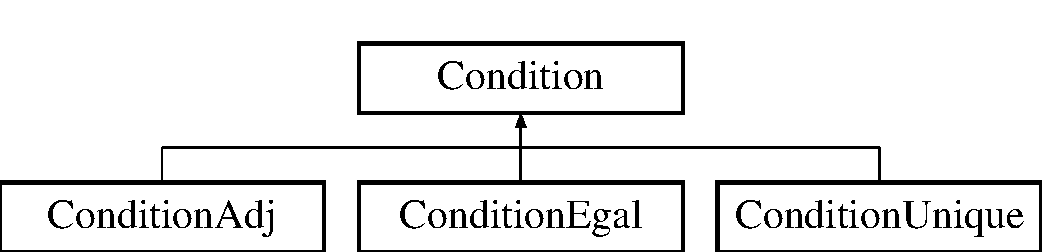
\includegraphics[height=2.000000cm]{class_condition}
\end{center}
\end{figure}
\subsection*{Attributs protégés}
\begin{DoxyCompactItemize}
\item 
\hypertarget{class_condition_a726c00e2c44548b135ea5c137ba836d2}{std\-::vector$<$ int $>$ {\bfseries indices}}\label{class_condition_a726c00e2c44548b135ea5c137ba836d2}

\end{DoxyCompactItemize}


La documentation de cette classe a été générée à partir du fichier suivant \-:\begin{DoxyCompactItemize}
\item 
grammaire/condition/Condition.\-h\end{DoxyCompactItemize}

\hypertarget{class_condition_adj}{\section{Référence de la classe Condition\-Adj}
\label{class_condition_adj}\index{Condition\-Adj@{Condition\-Adj}}
}
Graphe d'héritage de Condition\-Adj\-:\begin{figure}[H]
\begin{center}
\leavevmode
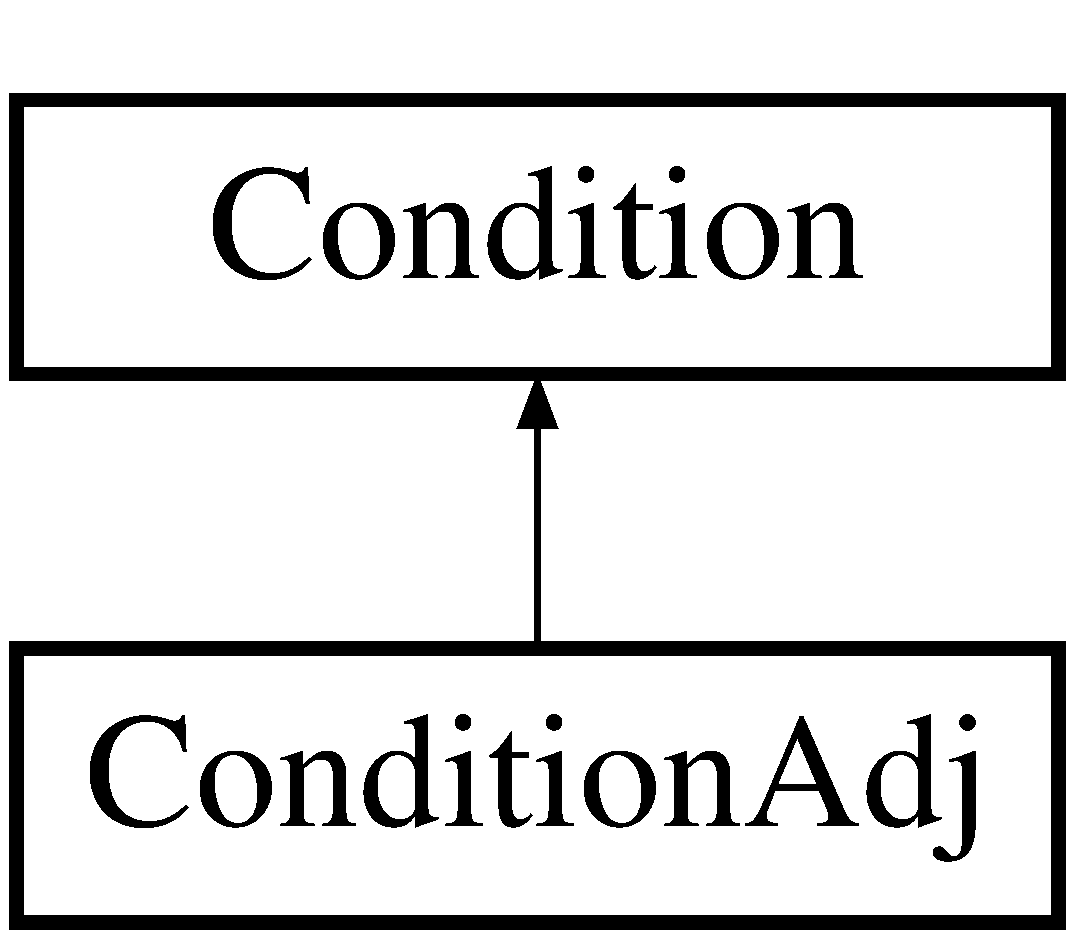
\includegraphics[height=2.000000cm]{class_condition_adj}
\end{center}
\end{figure}
\subsection*{Fonctions membres publiques}
\begin{DoxyCompactItemize}
\item 
\hypertarget{class_condition_adj_a02b8f6ba8554ab86cb1366b1a270de2c}{{\bfseries Condition\-Adj} (int i, string att\-\_\-i, int j, string att\-\_\-j)}\label{class_condition_adj_a02b8f6ba8554ab86cb1366b1a270de2c}

\end{DoxyCompactItemize}
\subsection*{Attributs publics}
\begin{DoxyCompactItemize}
\item 
\hypertarget{class_condition_adj_a337edb2f6c633335a19411a3db31ec36}{int {\bfseries i}}\label{class_condition_adj_a337edb2f6c633335a19411a3db31ec36}

\item 
\hypertarget{class_condition_adj_a00f7ccf764a7733e4c44eac8273abdad}{int {\bfseries j}}\label{class_condition_adj_a00f7ccf764a7733e4c44eac8273abdad}

\item 
\hypertarget{class_condition_adj_a45fa193bbab03993908bf29147cee704}{string {\bfseries att\-\_\-i}}\label{class_condition_adj_a45fa193bbab03993908bf29147cee704}

\item 
\hypertarget{class_condition_adj_a2a43d76fead9c535a4102a67dec08979}{string {\bfseries att\-\_\-j}}\label{class_condition_adj_a2a43d76fead9c535a4102a67dec08979}

\end{DoxyCompactItemize}


La documentation de cette classe a été générée à partir des fichiers suivants \-:\begin{DoxyCompactItemize}
\item 
grammaire/condition/Condition\-Adj.\-h\item 
grammaire/condition/Condition\-Adj.\-cpp\end{DoxyCompactItemize}

\hypertarget{class_condition_egal}{\section{Référence de la classe Condition\-Egal}
\label{class_condition_egal}\index{Condition\-Egal@{Condition\-Egal}}
}
Graphe d'héritage de Condition\-Egal\-:\begin{figure}[H]
\begin{center}
\leavevmode
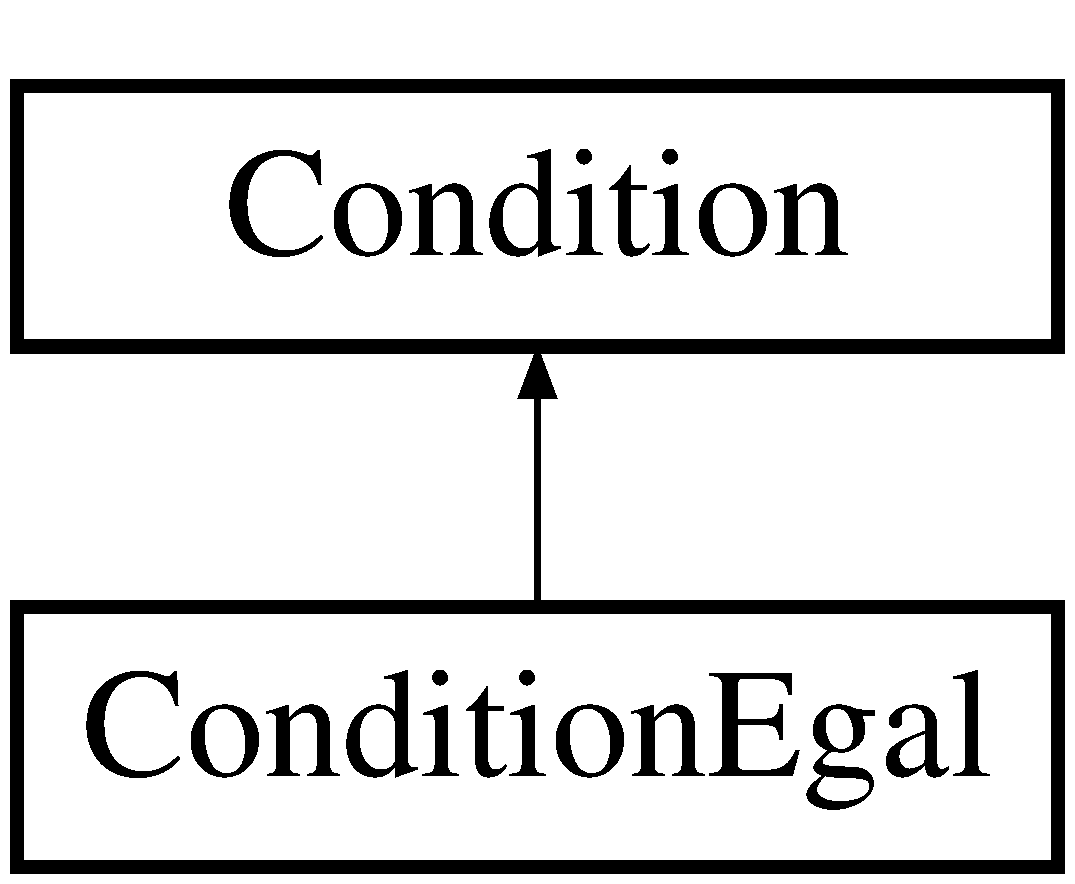
\includegraphics[height=2.000000cm]{class_condition_egal}
\end{center}
\end{figure}
\subsection*{Fonctions membres publiques}
\begin{DoxyCompactItemize}
\item 
\hypertarget{class_condition_egal_aca81c458365e1f76926d4be512612d4c}{{\bfseries Condition\-Egal} (int i, string att\-\_\-i, int j, string att\-\_\-j)}\label{class_condition_egal_aca81c458365e1f76926d4be512612d4c}

\end{DoxyCompactItemize}
\subsection*{Attributs publics}
\begin{DoxyCompactItemize}
\item 
\hypertarget{class_condition_egal_aeeee1cf74f01d9c42db0766b7e079668}{int {\bfseries i}}\label{class_condition_egal_aeeee1cf74f01d9c42db0766b7e079668}

\item 
\hypertarget{class_condition_egal_ae42bac38695763ad892b5c74e8d3b24f}{int {\bfseries j}}\label{class_condition_egal_ae42bac38695763ad892b5c74e8d3b24f}

\item 
\hypertarget{class_condition_egal_ae597fea6bf77fca3ba1e4d2d7a9d0e5d}{string {\bfseries att\-\_\-i}}\label{class_condition_egal_ae597fea6bf77fca3ba1e4d2d7a9d0e5d}

\item 
\hypertarget{class_condition_egal_a260aa94c917366bf38af15eaf8c46ade}{string {\bfseries att\-\_\-j}}\label{class_condition_egal_a260aa94c917366bf38af15eaf8c46ade}

\end{DoxyCompactItemize}


La documentation de cette classe a été générée à partir des fichiers suivants \-:\begin{DoxyCompactItemize}
\item 
grammaire/condition/Condition\-Egal.\-h\item 
grammaire/condition/Condition\-Egal.\-cpp\end{DoxyCompactItemize}

\hypertarget{class_condition_unique}{\section{Référence de la classe Condition\-Unique}
\label{class_condition_unique}\index{Condition\-Unique@{Condition\-Unique}}
}
Graphe d'héritage de Condition\-Unique\-:\begin{figure}[H]
\begin{center}
\leavevmode
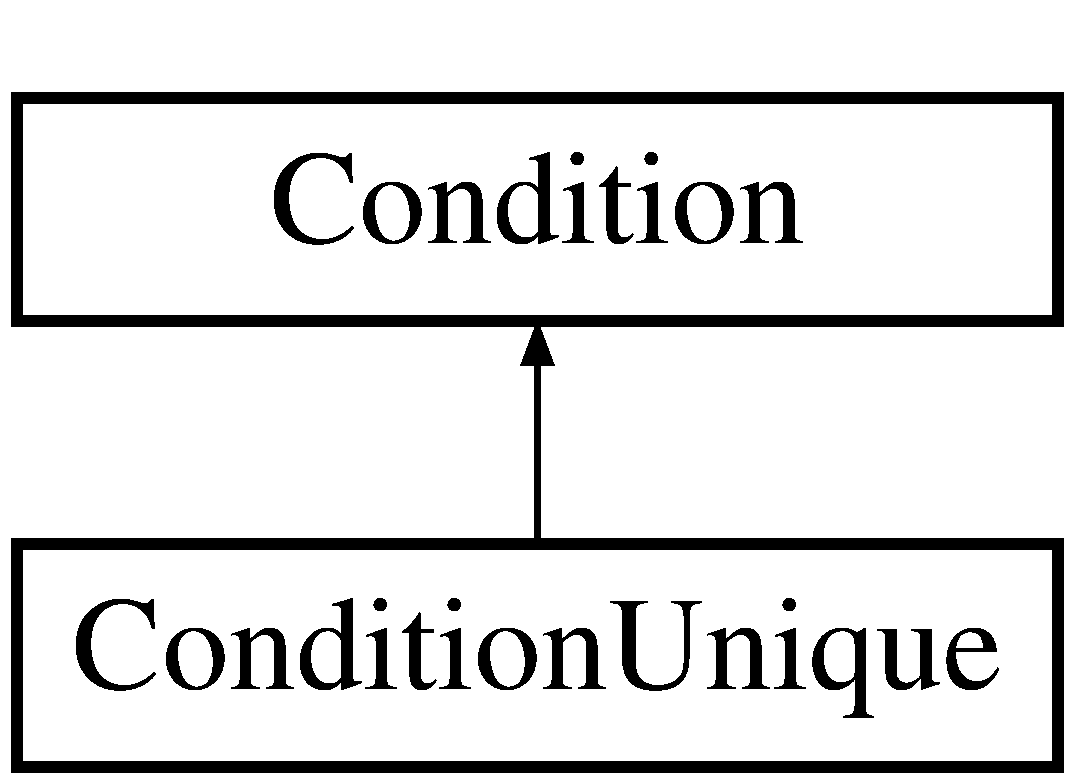
\includegraphics[height=2.000000cm]{class_condition_unique}
\end{center}
\end{figure}
\subsection*{Fonctions membres publiques}
\begin{DoxyCompactItemize}
\item 
\hypertarget{class_condition_unique_a6c0dde3aeaba3ecc47d7cbbc1b989015}{{\bfseries Condition\-Unique} (int i)}\label{class_condition_unique_a6c0dde3aeaba3ecc47d7cbbc1b989015}

\item 
\hypertarget{class_condition_unique_a6bf935dd0212e00c2ad83f25bddc091c}{virtual bool {\bfseries est\-Verifiee} (\hyperlink{class_noeud}{Noeud} $\ast$n)=0}\label{class_condition_unique_a6bf935dd0212e00c2ad83f25bddc091c}

\end{DoxyCompactItemize}
\subsection*{Attributs publics}
\begin{DoxyCompactItemize}
\item 
\hypertarget{class_condition_unique_ad629e86f3c6d9d8fdeedc7de1118e1ce}{int {\bfseries indice}}\label{class_condition_unique_ad629e86f3c6d9d8fdeedc7de1118e1ce}

\end{DoxyCompactItemize}


La documentation de cette classe a été générée à partir des fichiers suivants \-:\begin{DoxyCompactItemize}
\item 
grammaire/condition/Condition\-Unique.\-h\item 
grammaire/condition/Condition\-Unique.\-cpp\end{DoxyCompactItemize}

\hypertarget{class_convex_hull}{\section{Référence de la classe Convex\-Hull}
\label{class_convex_hull}\index{Convex\-Hull@{Convex\-Hull}}
}
Graphe d'héritage de Convex\-Hull\-:\begin{figure}[H]
\begin{center}
\leavevmode
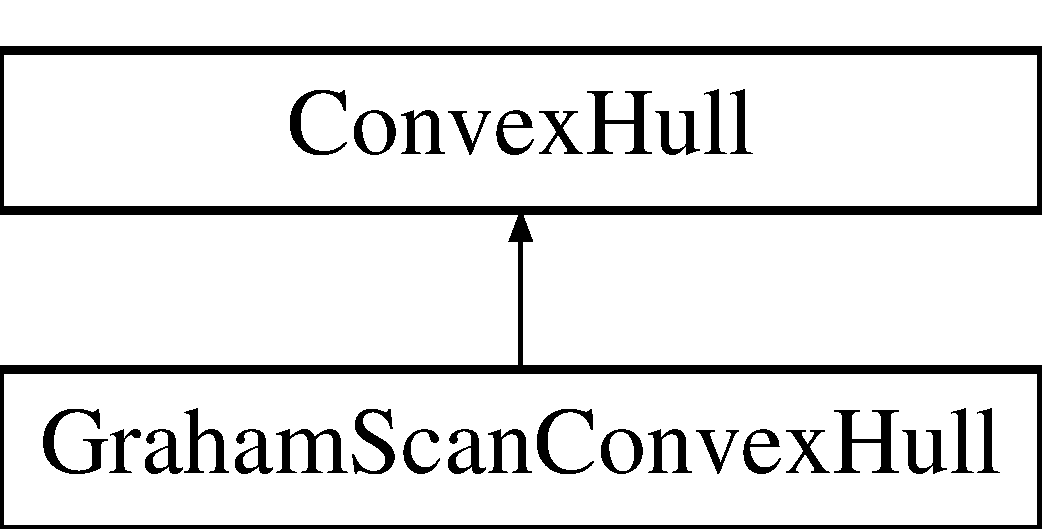
\includegraphics[height=2.000000cm]{class_convex_hull}
\end{center}
\end{figure}
\subsection*{Fonctions membres publiques}
\begin{DoxyCompactItemize}
\item 
\hypertarget{class_convex_hull_a21faf0ac7d97b87887afb40eb162ec65}{virtual bool {\bfseries operator()} (const std\-::vector$<$ \hyperlink{structpoint2d}{point2d} $>$ \&pnt, std\-::vector$<$ \hyperlink{structpoint2d}{point2d} $>$ \&final\-\_\-hull)=0}\label{class_convex_hull_a21faf0ac7d97b87887afb40eb162ec65}

\end{DoxyCompactItemize}


La documentation de cette classe a été générée à partir du fichier suivant \-:\begin{DoxyCompactItemize}
\item 
convexhull/Convex\-Hull.\-h\end{DoxyCompactItemize}

\hypertarget{class_convex_hull_e_p_s_writer}{\section{Référence de la classe Convex\-Hull\-E\-P\-S\-Writer}
\label{class_convex_hull_e_p_s_writer}\index{Convex\-Hull\-E\-P\-S\-Writer@{Convex\-Hull\-E\-P\-S\-Writer}}
}
\subsection*{Fonctions membres publiques}
\begin{DoxyCompactItemize}
\item 
\hypertarget{class_convex_hull_e_p_s_writer_a6d53dbdc0a4ff86fdb712b280b32e8b9}{bool {\bfseries operator()} (const std\-::string \&file\-\_\-name, const std\-::vector$<$ \hyperlink{structpoint2d}{point2d} $>$ \&point, const std\-::vector$<$ \hyperlink{structpoint2d}{point2d} $>$ \&hull)}\label{class_convex_hull_e_p_s_writer_a6d53dbdc0a4ff86fdb712b280b32e8b9}

\end{DoxyCompactItemize}
\subsection*{Fonctions membres privées}
\begin{DoxyCompactItemize}
\item 
\hypertarget{class_convex_hull_e_p_s_writer_a3b137bf654d760d8da0eefaf465f1b7a}{{\footnotesize template$<$typename T $>$ }\\std\-::string {\bfseries convert\-\_\-to\-\_\-string} (const T \&value)}\label{class_convex_hull_e_p_s_writer_a3b137bf654d760d8da0eefaf465f1b7a}

\end{DoxyCompactItemize}


La documentation de cette classe a été générée à partir du fichier suivant \-:\begin{DoxyCompactItemize}
\item 
convexhull/Convex\-Hull\-E\-P\-S\-Writer.\-h\end{DoxyCompactItemize}

\hypertarget{class_element}{\section{Référence de la classe Element}
\label{class_element}\index{Element@{Element}}
}
\subsection*{Fonctions membres publiques}
\begin{DoxyCompactItemize}
\item 
\hypertarget{class_element_a40db52eb2dc4be68ea32a8e4c021f3f6}{{\bfseries Element} (vector$<$ \hyperlink{class_noeud}{Noeud} $\ast$ $>$ membres, map$<$ string, void $\ast$ $>$ att\-\_\-debut, map$<$ string, void $\ast$ $>$ att\-\_\-fin)}\label{class_element_a40db52eb2dc4be68ea32a8e4c021f3f6}

\end{DoxyCompactItemize}
\subsection*{Attributs publics}
\begin{DoxyCompactItemize}
\item 
\hypertarget{class_element_a56902db0137ab191d92d1ae7bd5654ed}{vector$<$ \hyperlink{class_noeud}{Noeud} $\ast$ $>$ {\bfseries membres}}\label{class_element_a56902db0137ab191d92d1ae7bd5654ed}

\item 
\hypertarget{class_element_a167169b084f5ed44115c91e858f71f26}{map$<$ string, void $\ast$ $>$ {\bfseries att\-\_\-debut}}\label{class_element_a167169b084f5ed44115c91e858f71f26}

\item 
\hypertarget{class_element_a10c972e4b3c337135eda2064b70b869b}{map$<$ string, void $\ast$ $>$ {\bfseries att\-\_\-fin}}\label{class_element_a10c972e4b3c337135eda2064b70b869b}

\end{DoxyCompactItemize}


La documentation de cette classe a été générée à partir des fichiers suivants \-:\begin{DoxyCompactItemize}
\item 
grammaire/regles/Regle\-Sequence.\-h\item 
grammaire/regles/Regle\-Sequence.\-cpp\end{DoxyCompactItemize}

\hypertarget{class_graham_scan_convex_hull}{\section{Référence de la classe Graham\-Scan\-Convex\-Hull}
\label{class_graham_scan_convex_hull}\index{Graham\-Scan\-Convex\-Hull@{Graham\-Scan\-Convex\-Hull}}
}
Graphe d'héritage de Graham\-Scan\-Convex\-Hull\-:\begin{figure}[H]
\begin{center}
\leavevmode
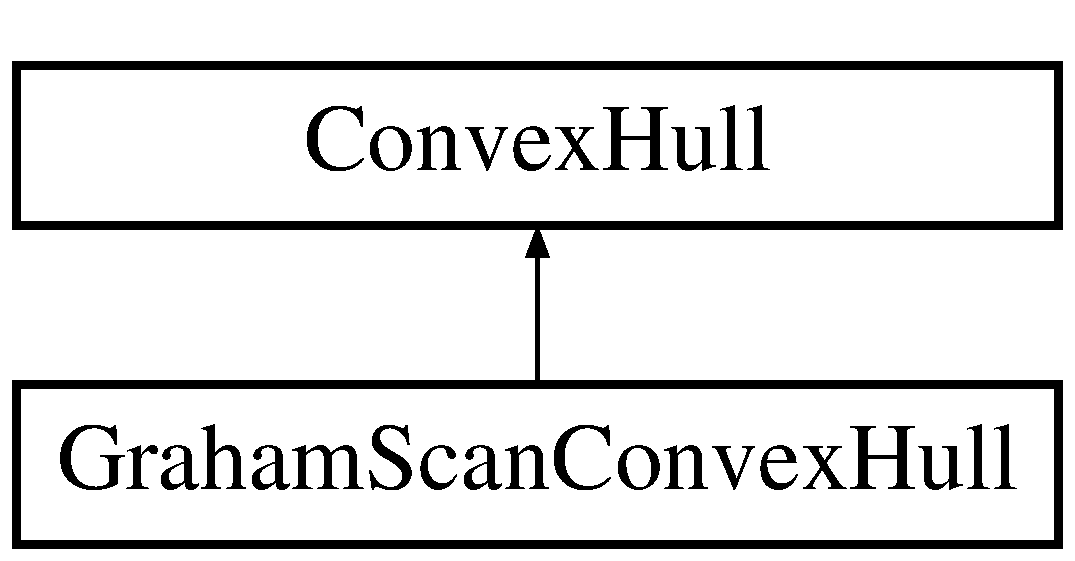
\includegraphics[height=2.000000cm]{class_graham_scan_convex_hull}
\end{center}
\end{figure}
\subsection*{Fonctions membres publiques}
\begin{DoxyCompactItemize}
\item 
\hypertarget{class_graham_scan_convex_hull_ac37484a57554ed7fe1c52b0e39f32986}{virtual bool {\bfseries operator()} (const std\-::vector$<$ \hyperlink{structpoint2d}{point2d} $>$ \&pnt, std\-::vector$<$ \hyperlink{structpoint2d}{point2d} $>$ \&final\-\_\-hull)}\label{class_graham_scan_convex_hull_ac37484a57554ed7fe1c52b0e39f32986}

\end{DoxyCompactItemize}
\subsection*{Fonctions membres privées}
\begin{DoxyCompactItemize}
\item 
\hypertarget{class_graham_scan_convex_hull_a393f7c83b7ffaef74c0970036b39578f}{void {\bfseries graham\-\_\-scan} (std\-::vector$<$ \hyperlink{structpoint2d}{point2d} $>$ \&final\-\_\-hull)}\label{class_graham_scan_convex_hull_a393f7c83b7ffaef74c0970036b39578f}

\item 
\hypertarget{class_graham_scan_convex_hull_ad965b00815fcfc087e6cf106bd93233f}{double {\bfseries cartesian\-\_\-angle} (double x, double y)}\label{class_graham_scan_convex_hull_ad965b00815fcfc087e6cf106bd93233f}

\item 
\hypertarget{class_graham_scan_convex_hull_a2b902769a85bb2dca1c255a9e11d5d47}{int {\bfseries orientation} (const \hyperlink{structgs__point2d}{gs\-\_\-point2d} \&p1, const \hyperlink{structgs__point2d}{gs\-\_\-point2d} \&p2, const \hyperlink{structgs__point2d}{gs\-\_\-point2d} \&p3)}\label{class_graham_scan_convex_hull_a2b902769a85bb2dca1c255a9e11d5d47}

\item 
\hypertarget{class_graham_scan_convex_hull_a6e3d1ea31abfc06bd47cc6feec394ecf}{int {\bfseries orientation} (const double x1, const double y1, const double x2, const double y2, const double px, const double py)}\label{class_graham_scan_convex_hull_a6e3d1ea31abfc06bd47cc6feec394ecf}

\item 
\hypertarget{class_graham_scan_convex_hull_a4eedb7210a8deea74ea028c33e08a9f8}{bool {\bfseries is\-\_\-equal} (const double v1, const double \&v2, const double epsilon=1.\-0e-\/12)}\label{class_graham_scan_convex_hull_a4eedb7210a8deea74ea028c33e08a9f8}

\end{DoxyCompactItemize}
\subsection*{Attributs privés}
\begin{DoxyCompactItemize}
\item 
\hypertarget{class_graham_scan_convex_hull_ab3176ef5d56ec8cae729676f4499dfaa}{std\-::vector$<$ \hyperlink{structgs__point2d}{gs\-\_\-point2d} $>$ {\bfseries point}}\label{class_graham_scan_convex_hull_ab3176ef5d56ec8cae729676f4499dfaa}

\item 
\hypertarget{class_graham_scan_convex_hull_ab2985c5e94ee951d00283af98b8ea6f0}{\hyperlink{structgs__point2d}{gs\-\_\-point2d} {\bfseries anchor}}\label{class_graham_scan_convex_hull_ab2985c5e94ee951d00283af98b8ea6f0}

\end{DoxyCompactItemize}


La documentation de cette classe a été générée à partir des fichiers suivants \-:\begin{DoxyCompactItemize}
\item 
convexhull/Graham\-Scan\-Convex\-Hull.\-h\item 
convexhull/Graham\-Scan\-Convex\-Hull.\-cpp\end{DoxyCompactItemize}

\hypertarget{structgs__point2d}{\section{Référence de la structure gs\-\_\-point2d}
\label{structgs__point2d}\index{gs\-\_\-point2d@{gs\-\_\-point2d}}
}
\subsection*{Fonctions membres publiques}
\begin{DoxyCompactItemize}
\item 
\hypertarget{structgs__point2d_a43686396b9d5c93398e3fc2c37d21937}{{\bfseries gs\-\_\-point2d} (double \-\_\-x=0.\-0, double \-\_\-y=0.\-0, double \-\_\-angle=0.\-0)}\label{structgs__point2d_a43686396b9d5c93398e3fc2c37d21937}

\end{DoxyCompactItemize}
\subsection*{Attributs publics}
\begin{DoxyCompactItemize}
\item 
\hypertarget{structgs__point2d_addfa94fc4fe707aadbf06129dbd475b7}{double {\bfseries x}}\label{structgs__point2d_addfa94fc4fe707aadbf06129dbd475b7}

\item 
\hypertarget{structgs__point2d_ac058f2b021a30e984483ae1a58fe78f5}{double {\bfseries y}}\label{structgs__point2d_ac058f2b021a30e984483ae1a58fe78f5}

\item 
\hypertarget{structgs__point2d_abcdef4d19a594e296c224f4a2bf23aac}{double {\bfseries angle}}\label{structgs__point2d_abcdef4d19a594e296c224f4a2bf23aac}

\end{DoxyCompactItemize}


La documentation de cette structure a été générée à partir du fichier suivant \-:\begin{DoxyCompactItemize}
\item 
convexhull/Graham\-Scan\-Convex\-Hull.\-h\end{DoxyCompactItemize}

\hypertarget{class_g_s_point2_d_compare}{\section{Référence de la classe G\-S\-Point2\-D\-Compare}
\label{class_g_s_point2_d_compare}\index{G\-S\-Point2\-D\-Compare@{G\-S\-Point2\-D\-Compare}}
}
\subsection*{Fonctions membres publiques}
\begin{DoxyCompactItemize}
\item 
\hypertarget{class_g_s_point2_d_compare_a5f1ee29c548143850250ba4ff2a020a7}{{\bfseries G\-S\-Point2\-D\-Compare} (\hyperlink{structgs__point2d}{gs\-\_\-point2d} $\ast$\-\_\-anchor)}\label{class_g_s_point2_d_compare_a5f1ee29c548143850250ba4ff2a020a7}

\item 
\hypertarget{class_g_s_point2_d_compare_af1b994734c1817514087cd9d6a67341c}{bool {\bfseries operator()} (const \hyperlink{structgs__point2d}{gs\-\_\-point2d} \&p1, const \hyperlink{structgs__point2d}{gs\-\_\-point2d} \&p2)}\label{class_g_s_point2_d_compare_af1b994734c1817514087cd9d6a67341c}

\end{DoxyCompactItemize}
\subsection*{Fonctions membres privées}
\begin{DoxyCompactItemize}
\item 
\hypertarget{class_g_s_point2_d_compare_a79297396ba1d7e1b38c3ade487d1ccaf}{bool {\bfseries is\-\_\-equal} (const \hyperlink{structgs__point2d}{gs\-\_\-point2d} p1, \hyperlink{structgs__point2d}{gs\-\_\-point2d} p2)}\label{class_g_s_point2_d_compare_a79297396ba1d7e1b38c3ade487d1ccaf}

\item 
\hypertarget{class_g_s_point2_d_compare_a758a2bab4f965fbc52250d26e737f835}{bool {\bfseries is\-\_\-equal} (const double v1, const double \&v2, const double epsilon=1.\-0e-\/12)}\label{class_g_s_point2_d_compare_a758a2bab4f965fbc52250d26e737f835}

\item 
\hypertarget{class_g_s_point2_d_compare_aeff7984846aa78602f68eaea28b173dc}{double {\bfseries lay\-\_\-distance} (const double \&x1, const double \&y1, const double \&x2, const double \&y2)}\label{class_g_s_point2_d_compare_aeff7984846aa78602f68eaea28b173dc}

\end{DoxyCompactItemize}
\subsection*{Attributs privés}
\begin{DoxyCompactItemize}
\item 
\hypertarget{class_g_s_point2_d_compare_a6565ae0a6cb40a412f5e72558ed3271f}{\hyperlink{structgs__point2d}{gs\-\_\-point2d} $\ast$ {\bfseries anchor}}\label{class_g_s_point2_d_compare_a6565ae0a6cb40a412f5e72558ed3271f}

\end{DoxyCompactItemize}


La documentation de cette classe a été générée à partir du fichier suivant \-:\begin{DoxyCompactItemize}
\item 
convexhull/Graham\-Scan\-Convex\-Hull.\-h\end{DoxyCompactItemize}

\hypertarget{structlist}{\section{Référence de la structure list}
\label{structlist}\index{list@{list}}
}
\subsection*{Attributs publics}
\begin{DoxyCompactItemize}
\item 
\hypertarget{structlist_a1e4f9682bfdc33db2d825fd41658a88d}{int {\bfseries item\-\_\-count}}\label{structlist_a1e4f9682bfdc33db2d825fd41658a88d}

\item 
\hypertarget{structlist_af13cdd9f7d31327fc22ed5da5623aa27}{int {\bfseries current\-\_\-max\-\_\-size}}\label{structlist_af13cdd9f7d31327fc22ed5da5623aa27}

\item 
\hypertarget{structlist_a7da9bddee81290f233d7ec41f26824f3}{char {\bfseries growable}}\label{structlist_a7da9bddee81290f233d7ec41f26824f3}

\item 
\hypertarget{structlist_ade0b0790a7fd4f3b65aae379d5a7da85}{void $\ast$$\ast$ {\bfseries items}}\label{structlist_ade0b0790a7fd4f3b65aae379d5a7da85}

\item 
\hypertarget{structlist_a1b3f452b7de983fc5b841f4569285e57}{char $\ast$$\ast$ {\bfseries names}}\label{structlist_a1b3f452b7de983fc5b841f4569285e57}

\end{DoxyCompactItemize}


La documentation de cette structure a été générée à partir du fichier suivant \-:\begin{DoxyCompactItemize}
\item 
obj\-Loader/list.\-h\end{DoxyCompactItemize}

\hypertarget{class_matrice2}{\section{Référence de la classe Matrice2}
\label{class_matrice2}\index{Matrice2@{Matrice2}}
}
\subsection*{Fonctions membres publiques}
\begin{DoxyCompactItemize}
\item 
\hypertarget{class_matrice2_a83a70ba4858f14e89c5287ec59ae96d0}{{\bfseries Matrice2} (float a, float b, float c, float d)}\label{class_matrice2_a83a70ba4858f14e89c5287ec59ae96d0}

\item 
\hypertarget{class_matrice2_a4a5e8561a8616485fc492ec569429eb2}{\hyperlink{class_matrice2}{Matrice2} $\ast$ {\bfseries transpose} ()}\label{class_matrice2_a4a5e8561a8616485fc492ec569429eb2}

\end{DoxyCompactItemize}
\subsection*{Attributs publics}
\begin{DoxyCompactItemize}
\item 
\hypertarget{class_matrice2_aa249f4f1243999d731ab48889272cb70}{float $\ast$$\ast$ {\bfseries mat}}\label{class_matrice2_aa249f4f1243999d731ab48889272cb70}

\end{DoxyCompactItemize}
\subsection*{Fonctions membres privées}
\begin{DoxyCompactItemize}
\item 
\hypertarget{class_matrice2_a04fc6ee0ed98d9a76cb6fffb8ea52168}{void {\bfseries init} ()}\label{class_matrice2_a04fc6ee0ed98d9a76cb6fffb8ea52168}

\end{DoxyCompactItemize}


La documentation de cette classe a été générée à partir des fichiers suivants \-:\begin{DoxyCompactItemize}
\item 
geometrie/Matrice2.\-h\item 
geometrie/Matrice2.\-cpp\end{DoxyCompactItemize}

\hypertarget{class_noeud}{\section{Référence de la classe Noeud}
\label{class_noeud}\index{Noeud@{Noeud}}
}
Graphe d'héritage de Noeud\-:\begin{figure}[H]
\begin{center}
\leavevmode
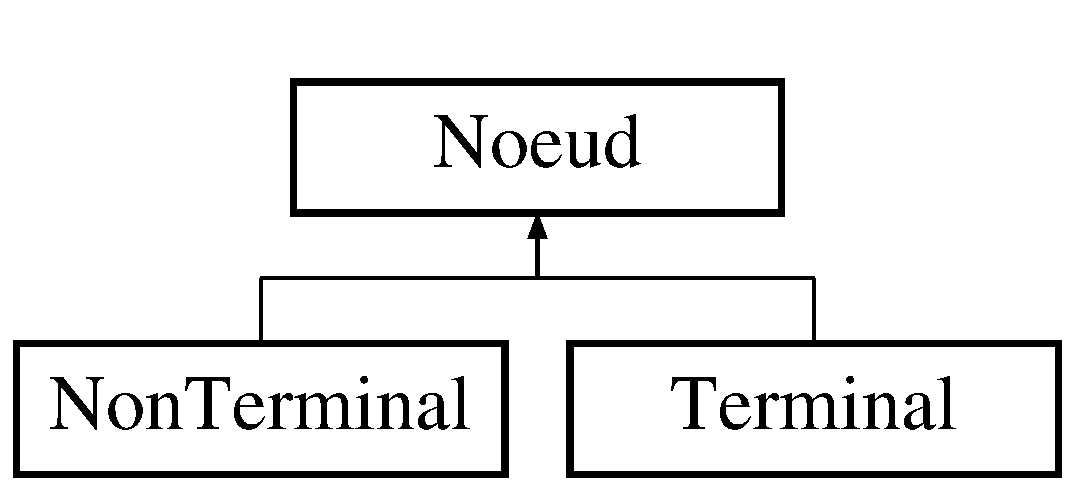
\includegraphics[height=2.000000cm]{class_noeud}
\end{center}
\end{figure}
\subsection*{Fonctions membres publiques}
\begin{DoxyCompactItemize}
\item 
\hypertarget{class_noeud_ab9d96398e3e1c4767c83110463d130df}{virtual vector$<$ \hyperlink{class_noeud}{Noeud} $\ast$ $>$ {\bfseries get\-Enfants} ()=0}\label{class_noeud_ab9d96398e3e1c4767c83110463d130df}

\item 
\hypertarget{class_noeud_a23ab9345dad17e61c1891a8e5660df60}{virtual string {\bfseries get\-Type} ()=0}\label{class_noeud_a23ab9345dad17e61c1891a8e5660df60}

\item 
\hypertarget{class_noeud_ac36be22327cdf8872e8f61ed0d14d16b}{void $\ast$ {\bfseries get\-Attribut} (string nom)}\label{class_noeud_ac36be22327cdf8872e8f61ed0d14d16b}

\item 
\hypertarget{class_noeud_a235fd45cbeb5cbf2837cc69c470f3dcf}{map$<$ string, void $\ast$ $>$ {\bfseries get\-Attributs} ()}\label{class_noeud_a235fd45cbeb5cbf2837cc69c470f3dcf}

\item 
\hypertarget{class_noeud_a8b34dbe57ecb402eca805ef0bc895d66}{void {\bfseries set\-Attribut} (string nom, void $\ast$val)}\label{class_noeud_a8b34dbe57ecb402eca805ef0bc895d66}

\item 
\hypertarget{class_noeud_a5268b4941c341393d746653f9a991672}{virtual bool {\bfseries equals} (\hyperlink{class_noeud}{Noeud} $\ast$n2)=0}\label{class_noeud_a5268b4941c341393d746653f9a991672}

\end{DoxyCompactItemize}
\subsection*{Attributs protégés}
\begin{DoxyCompactItemize}
\item 
\hypertarget{class_noeud_a7eff1e9588e1ee40671ce7d8497db140}{map$<$ string, void $\ast$ $>$ {\bfseries attributs}}\label{class_noeud_a7eff1e9588e1ee40671ce7d8497db140}

\end{DoxyCompactItemize}


La documentation de cette classe a été générée à partir des fichiers suivants \-:\begin{DoxyCompactItemize}
\item 
grammaire/parsing/Noeud.\-h\item 
grammaire/parsing/Noeud.\-cpp\end{DoxyCompactItemize}

\hypertarget{class_non_terminal}{\section{Référence de la classe Non\-Terminal}
\label{class_non_terminal}\index{Non\-Terminal@{Non\-Terminal}}
}
Graphe d'héritage de Non\-Terminal\-:\begin{figure}[H]
\begin{center}
\leavevmode
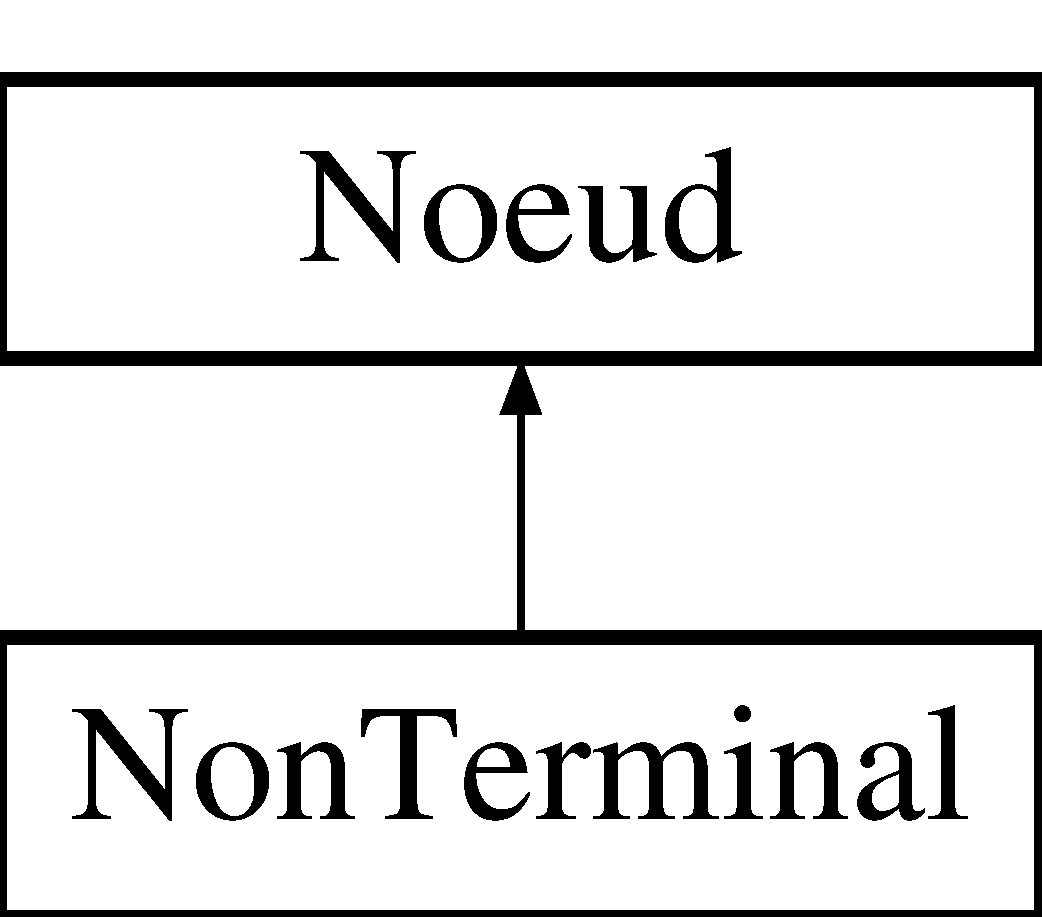
\includegraphics[height=2.000000cm]{class_non_terminal}
\end{center}
\end{figure}
\subsection*{Fonctions membres publiques}
\begin{DoxyCompactItemize}
\item 
\hypertarget{class_non_terminal_a71519a9ddb6a0ca896360a09cc2c612e}{{\bfseries Non\-Terminal} (string type, vector$<$ \hyperlink{class_noeud}{Noeud} $\ast$ $>$ enfants)}\label{class_non_terminal_a71519a9ddb6a0ca896360a09cc2c612e}

\item 
\hypertarget{class_non_terminal_ac1a9b3b1dcd715b6889d615354d4ae1b}{vector$<$ \hyperlink{class_noeud}{Noeud} $\ast$ $>$ {\bfseries get\-Enfants} ()}\label{class_non_terminal_ac1a9b3b1dcd715b6889d615354d4ae1b}

\item 
\hypertarget{class_non_terminal_abb05a6a5e8850c55deb08a33d665a588}{string {\bfseries get\-Type} ()}\label{class_non_terminal_abb05a6a5e8850c55deb08a33d665a588}

\item 
\hypertarget{class_non_terminal_ad1871090f16d09962e99fc02f5f28e1f}{bool {\bfseries equals} (\hyperlink{class_noeud}{Noeud} $\ast$n)}\label{class_non_terminal_ad1871090f16d09962e99fc02f5f28e1f}

\end{DoxyCompactItemize}
\subsection*{Attributs privés}
\begin{DoxyCompactItemize}
\item 
\hypertarget{class_non_terminal_a74245dee79b2ef98bcd75c10c25e79c0}{vector$<$ \hyperlink{class_noeud}{Noeud} $\ast$ $>$ {\bfseries enfants}}\label{class_non_terminal_a74245dee79b2ef98bcd75c10c25e79c0}

\item 
\hypertarget{class_non_terminal_a3a7aed08c66e46f67ef0a1f532a3b83c}{string {\bfseries type}}\label{class_non_terminal_a3a7aed08c66e46f67ef0a1f532a3b83c}

\end{DoxyCompactItemize}


La documentation de cette classe a été générée à partir des fichiers suivants \-:\begin{DoxyCompactItemize}
\item 
grammaire/parsing/Non\-Terminal.\-h\item 
grammaire/parsing/Non\-Terminal.\-cpp\end{DoxyCompactItemize}

\hypertarget{structobj__camera}{\section{Référence de la structure obj\-\_\-camera}
\label{structobj__camera}\index{obj\-\_\-camera@{obj\-\_\-camera}}
}
\subsection*{Attributs publics}
\begin{DoxyCompactItemize}
\item 
\hypertarget{structobj__camera_a02c5e1c127fc81b0377d773572d82a8a}{int {\bfseries camera\-\_\-pos\-\_\-index}}\label{structobj__camera_a02c5e1c127fc81b0377d773572d82a8a}

\item 
\hypertarget{structobj__camera_ad795a90bb5ddd7298fac17af40317881}{int {\bfseries camera\-\_\-look\-\_\-point\-\_\-index}}\label{structobj__camera_ad795a90bb5ddd7298fac17af40317881}

\item 
\hypertarget{structobj__camera_a2d8ae90adcf03df3b2b28c3c13e1da5d}{int {\bfseries camera\-\_\-up\-\_\-norm\-\_\-index}}\label{structobj__camera_a2d8ae90adcf03df3b2b28c3c13e1da5d}

\end{DoxyCompactItemize}


La documentation de cette structure a été générée à partir du fichier suivant \-:\begin{DoxyCompactItemize}
\item 
obj\-Loader/obj\-\_\-parser.\-h\end{DoxyCompactItemize}

\hypertarget{structobj__face}{\section{Référence de la structure obj\-\_\-face}
\label{structobj__face}\index{obj\-\_\-face@{obj\-\_\-face}}
}
\subsection*{Attributs publics}
\begin{DoxyCompactItemize}
\item 
\hypertarget{structobj__face_a507982facfb73bcd3143d962e8aba781}{int {\bfseries vertex\-\_\-index} \mbox{[}M\-A\-X\-\_\-\-V\-E\-R\-T\-E\-X\-\_\-\-C\-O\-U\-N\-T\mbox{]}}\label{structobj__face_a507982facfb73bcd3143d962e8aba781}

\item 
\hypertarget{structobj__face_aa37ed96ceb21dde7ca0e07436f0c60bd}{int {\bfseries normal\-\_\-index} \mbox{[}M\-A\-X\-\_\-\-V\-E\-R\-T\-E\-X\-\_\-\-C\-O\-U\-N\-T\mbox{]}}\label{structobj__face_aa37ed96ceb21dde7ca0e07436f0c60bd}

\item 
\hypertarget{structobj__face_affde6e39f099c5f3497c3691ea66608c}{int {\bfseries texture\-\_\-index} \mbox{[}M\-A\-X\-\_\-\-V\-E\-R\-T\-E\-X\-\_\-\-C\-O\-U\-N\-T\mbox{]}}\label{structobj__face_affde6e39f099c5f3497c3691ea66608c}

\item 
\hypertarget{structobj__face_ac1a658f759cfb36b241a013cce1a8744}{int {\bfseries vertex\-\_\-count}}\label{structobj__face_ac1a658f759cfb36b241a013cce1a8744}

\item 
\hypertarget{structobj__face_ab354e6f87c96bd040a9cd6d4c4532f6b}{int {\bfseries material\-\_\-index}}\label{structobj__face_ab354e6f87c96bd040a9cd6d4c4532f6b}

\end{DoxyCompactItemize}


La documentation de cette structure a été générée à partir du fichier suivant \-:\begin{DoxyCompactItemize}
\item 
obj\-Loader/obj\-\_\-parser.\-h\end{DoxyCompactItemize}

\hypertarget{structobj__growable__scene__data}{\section{Référence de la structure obj\-\_\-growable\-\_\-scene\-\_\-data}
\label{structobj__growable__scene__data}\index{obj\-\_\-growable\-\_\-scene\-\_\-data@{obj\-\_\-growable\-\_\-scene\-\_\-data}}
}
\subsection*{Attributs publics}
\begin{DoxyCompactItemize}
\item 
\hypertarget{structobj__growable__scene__data_ab11f689f063e184661781e94da0ccce1}{char {\bfseries scene\-\_\-filename} \mbox{[}O\-B\-J\-\_\-\-F\-I\-L\-E\-N\-A\-M\-E\-\_\-\-L\-E\-N\-G\-T\-H\mbox{]}}\label{structobj__growable__scene__data_ab11f689f063e184661781e94da0ccce1}

\item 
\hypertarget{structobj__growable__scene__data_a2b760bb727ab7b49bb9971fb3e6ed3a8}{char {\bfseries material\-\_\-filename} \mbox{[}O\-B\-J\-\_\-\-F\-I\-L\-E\-N\-A\-M\-E\-\_\-\-L\-E\-N\-G\-T\-H\mbox{]}}\label{structobj__growable__scene__data_a2b760bb727ab7b49bb9971fb3e6ed3a8}

\item 
\hypertarget{structobj__growable__scene__data_a13975a6dbaa62718add1043de08324d8}{\hyperlink{structlist}{list} {\bfseries vertex\-\_\-list}}\label{structobj__growable__scene__data_a13975a6dbaa62718add1043de08324d8}

\item 
\hypertarget{structobj__growable__scene__data_a8434f1f1123eaf06a4e87f7a4c157527}{\hyperlink{structlist}{list} {\bfseries vertex\-\_\-normal\-\_\-list}}\label{structobj__growable__scene__data_a8434f1f1123eaf06a4e87f7a4c157527}

\item 
\hypertarget{structobj__growable__scene__data_a85ee455560d2f8c8910257bb4b96c5bf}{\hyperlink{structlist}{list} {\bfseries vertex\-\_\-texture\-\_\-list}}\label{structobj__growable__scene__data_a85ee455560d2f8c8910257bb4b96c5bf}

\item 
\hypertarget{structobj__growable__scene__data_a371039f614baf3b51c079d577ed8247a}{\hyperlink{structlist}{list} {\bfseries face\-\_\-list}}\label{structobj__growable__scene__data_a371039f614baf3b51c079d577ed8247a}

\item 
\hypertarget{structobj__growable__scene__data_a5c49ed985e0f8bddf535807b840618f3}{\hyperlink{structlist}{list} {\bfseries sphere\-\_\-list}}\label{structobj__growable__scene__data_a5c49ed985e0f8bddf535807b840618f3}

\item 
\hypertarget{structobj__growable__scene__data_aea6999082b6a4000f5753ab81e30806b}{\hyperlink{structlist}{list} {\bfseries plane\-\_\-list}}\label{structobj__growable__scene__data_aea6999082b6a4000f5753ab81e30806b}

\item 
\hypertarget{structobj__growable__scene__data_a78cb39927508e8622f328756a954c50d}{\hyperlink{structlist}{list} {\bfseries light\-\_\-point\-\_\-list}}\label{structobj__growable__scene__data_a78cb39927508e8622f328756a954c50d}

\item 
\hypertarget{structobj__growable__scene__data_a64d1574b4bae19b123e8cb3f6688555f}{\hyperlink{structlist}{list} {\bfseries light\-\_\-quad\-\_\-list}}\label{structobj__growable__scene__data_a64d1574b4bae19b123e8cb3f6688555f}

\item 
\hypertarget{structobj__growable__scene__data_a774c6e71151e61488452babc59db667c}{\hyperlink{structlist}{list} {\bfseries light\-\_\-disc\-\_\-list}}\label{structobj__growable__scene__data_a774c6e71151e61488452babc59db667c}

\item 
\hypertarget{structobj__growable__scene__data_ad271be9b71b2dfd6fbadd5bf69e74bf5}{\hyperlink{structlist}{list} {\bfseries material\-\_\-list}}\label{structobj__growable__scene__data_ad271be9b71b2dfd6fbadd5bf69e74bf5}

\item 
\hypertarget{structobj__growable__scene__data_a44df213a8051ff348dbeba280ee7112c}{\hyperlink{structobj__camera}{obj\-\_\-camera} $\ast$ {\bfseries camera}}\label{structobj__growable__scene__data_a44df213a8051ff348dbeba280ee7112c}

\end{DoxyCompactItemize}


La documentation de cette structure a été générée à partir du fichier suivant \-:\begin{DoxyCompactItemize}
\item 
obj\-Loader/obj\-\_\-parser.\-h\end{DoxyCompactItemize}

\hypertarget{structobj__light__disc}{\section{Référence de la structure obj\-\_\-light\-\_\-disc}
\label{structobj__light__disc}\index{obj\-\_\-light\-\_\-disc@{obj\-\_\-light\-\_\-disc}}
}
\subsection*{Attributs publics}
\begin{DoxyCompactItemize}
\item 
\hypertarget{structobj__light__disc_a06e88be817f6fc3b1ad8338a05d004db}{int {\bfseries pos\-\_\-index}}\label{structobj__light__disc_a06e88be817f6fc3b1ad8338a05d004db}

\item 
\hypertarget{structobj__light__disc_abff6571d08e00cab1cf246b460487076}{int {\bfseries normal\-\_\-index}}\label{structobj__light__disc_abff6571d08e00cab1cf246b460487076}

\item 
\hypertarget{structobj__light__disc_ab3f2c2e21bdda9da7efb82e9fb250cb0}{int {\bfseries material\-\_\-index}}\label{structobj__light__disc_ab3f2c2e21bdda9da7efb82e9fb250cb0}

\end{DoxyCompactItemize}


La documentation de cette structure a été générée à partir du fichier suivant \-:\begin{DoxyCompactItemize}
\item 
obj\-Loader/obj\-\_\-parser.\-h\end{DoxyCompactItemize}

\hypertarget{structobj__light__point}{\section{Référence de la structure obj\-\_\-light\-\_\-point}
\label{structobj__light__point}\index{obj\-\_\-light\-\_\-point@{obj\-\_\-light\-\_\-point}}
}
\subsection*{Attributs publics}
\begin{DoxyCompactItemize}
\item 
\hypertarget{structobj__light__point_af1cc014add4a2347bfe42c679b045a33}{int {\bfseries pos\-\_\-index}}\label{structobj__light__point_af1cc014add4a2347bfe42c679b045a33}

\item 
\hypertarget{structobj__light__point_af1b77673d08020affbb95e3f0bf75f4a}{int {\bfseries material\-\_\-index}}\label{structobj__light__point_af1b77673d08020affbb95e3f0bf75f4a}

\end{DoxyCompactItemize}


La documentation de cette structure a été générée à partir du fichier suivant \-:\begin{DoxyCompactItemize}
\item 
obj\-Loader/obj\-\_\-parser.\-h\end{DoxyCompactItemize}

\hypertarget{structobj__light__quad}{\section{Référence de la structure obj\-\_\-light\-\_\-quad}
\label{structobj__light__quad}\index{obj\-\_\-light\-\_\-quad@{obj\-\_\-light\-\_\-quad}}
}
\subsection*{Attributs publics}
\begin{DoxyCompactItemize}
\item 
\hypertarget{structobj__light__quad_a1ed9f7f7a517ab90f2b8c6b515f3654e}{int {\bfseries vertex\-\_\-index} \mbox{[}M\-A\-X\-\_\-\-V\-E\-R\-T\-E\-X\-\_\-\-C\-O\-U\-N\-T\mbox{]}}\label{structobj__light__quad_a1ed9f7f7a517ab90f2b8c6b515f3654e}

\item 
\hypertarget{structobj__light__quad_ad12afb43f3ca35ebd6c6e3a81063edb2}{int {\bfseries material\-\_\-index}}\label{structobj__light__quad_ad12afb43f3ca35ebd6c6e3a81063edb2}

\end{DoxyCompactItemize}


La documentation de cette structure a été générée à partir du fichier suivant \-:\begin{DoxyCompactItemize}
\item 
obj\-Loader/obj\-\_\-parser.\-h\end{DoxyCompactItemize}

\hypertarget{structobj__material}{\section{Référence de la structure obj\-\_\-material}
\label{structobj__material}\index{obj\-\_\-material@{obj\-\_\-material}}
}
\subsection*{Attributs publics}
\begin{DoxyCompactItemize}
\item 
\hypertarget{structobj__material_a22c868555082c2637cef0515b5a7ca6b}{char {\bfseries name} \mbox{[}M\-A\-T\-E\-R\-I\-A\-L\-\_\-\-N\-A\-M\-E\-\_\-\-S\-I\-Z\-E\mbox{]}}\label{structobj__material_a22c868555082c2637cef0515b5a7ca6b}

\item 
\hypertarget{structobj__material_a432c6437ac6a50152c553684fab0aaef}{char {\bfseries texture\-\_\-filename} \mbox{[}O\-B\-J\-\_\-\-F\-I\-L\-E\-N\-A\-M\-E\-\_\-\-L\-E\-N\-G\-T\-H\mbox{]}}\label{structobj__material_a432c6437ac6a50152c553684fab0aaef}

\item 
\hypertarget{structobj__material_a0127f4464e685658f8bf9db697688f8d}{double {\bfseries amb} \mbox{[}3\mbox{]}}\label{structobj__material_a0127f4464e685658f8bf9db697688f8d}

\item 
\hypertarget{structobj__material_a6f9b724555e48815e800b4f82c291f19}{double {\bfseries diff} \mbox{[}3\mbox{]}}\label{structobj__material_a6f9b724555e48815e800b4f82c291f19}

\item 
\hypertarget{structobj__material_aaba883a6684bc146f396a39534e5ae57}{double {\bfseries spec} \mbox{[}3\mbox{]}}\label{structobj__material_aaba883a6684bc146f396a39534e5ae57}

\item 
\hypertarget{structobj__material_a4763ba95918c9bf5256b79e3603adc58}{double {\bfseries reflect}}\label{structobj__material_a4763ba95918c9bf5256b79e3603adc58}

\item 
\hypertarget{structobj__material_a322daa5a65bd76d646dea59bf93e29c0}{double {\bfseries refract}}\label{structobj__material_a322daa5a65bd76d646dea59bf93e29c0}

\item 
\hypertarget{structobj__material_adfe718fbbdb972e83b4159d4c634b14b}{double {\bfseries trans}}\label{structobj__material_adfe718fbbdb972e83b4159d4c634b14b}

\item 
\hypertarget{structobj__material_aa238fbf38e7eadb10ceed02324213d5d}{double {\bfseries shiny}}\label{structobj__material_aa238fbf38e7eadb10ceed02324213d5d}

\item 
\hypertarget{structobj__material_a9d648bad424ee96576ed2a2f2e604da6}{double {\bfseries glossy}}\label{structobj__material_a9d648bad424ee96576ed2a2f2e604da6}

\item 
\hypertarget{structobj__material_a6931b83a6b1e681d094751258189259b}{double {\bfseries refract\-\_\-index}}\label{structobj__material_a6931b83a6b1e681d094751258189259b}

\end{DoxyCompactItemize}


La documentation de cette structure a été générée à partir du fichier suivant \-:\begin{DoxyCompactItemize}
\item 
obj\-Loader/obj\-\_\-parser.\-h\end{DoxyCompactItemize}

\hypertarget{structobj__plane}{\section{Référence de la structure obj\-\_\-plane}
\label{structobj__plane}\index{obj\-\_\-plane@{obj\-\_\-plane}}
}
\subsection*{Attributs publics}
\begin{DoxyCompactItemize}
\item 
\hypertarget{structobj__plane_abaa3eff0fff8deaa67eb4be6869b7048}{int {\bfseries pos\-\_\-index}}\label{structobj__plane_abaa3eff0fff8deaa67eb4be6869b7048}

\item 
\hypertarget{structobj__plane_acf720ed71df9e09ab0797d61ffdf7663}{int {\bfseries normal\-\_\-index}}\label{structobj__plane_acf720ed71df9e09ab0797d61ffdf7663}

\item 
\hypertarget{structobj__plane_a0c0c054b3a747f4ec2486fdf367efa36}{int {\bfseries rotation\-\_\-normal\-\_\-index}}\label{structobj__plane_a0c0c054b3a747f4ec2486fdf367efa36}

\item 
\hypertarget{structobj__plane_a38a87ad9ef6583b136c8438c2bd4229b}{int {\bfseries texture\-\_\-index} \mbox{[}M\-A\-X\-\_\-\-V\-E\-R\-T\-E\-X\-\_\-\-C\-O\-U\-N\-T\mbox{]}}\label{structobj__plane_a38a87ad9ef6583b136c8438c2bd4229b}

\item 
\hypertarget{structobj__plane_ae0783771277bc7c8b2b8743015104291}{int {\bfseries material\-\_\-index}}\label{structobj__plane_ae0783771277bc7c8b2b8743015104291}

\end{DoxyCompactItemize}


La documentation de cette structure a été générée à partir du fichier suivant \-:\begin{DoxyCompactItemize}
\item 
obj\-Loader/obj\-\_\-parser.\-h\end{DoxyCompactItemize}

\hypertarget{structobj__scene__data}{\section{Référence de la structure obj\-\_\-scene\-\_\-data}
\label{structobj__scene__data}\index{obj\-\_\-scene\-\_\-data@{obj\-\_\-scene\-\_\-data}}
}
\subsection*{Attributs publics}
\begin{DoxyCompactItemize}
\item 
\hypertarget{structobj__scene__data_ae63c9e7899791d0ac616aab05d2a3d55}{\hyperlink{structobj__vector}{obj\-\_\-vector} $\ast$$\ast$ {\bfseries vertex\-\_\-list}}\label{structobj__scene__data_ae63c9e7899791d0ac616aab05d2a3d55}

\item 
\hypertarget{structobj__scene__data_a8407af16c78de18ecb879dc627109560}{\hyperlink{structobj__vector}{obj\-\_\-vector} $\ast$$\ast$ {\bfseries vertex\-\_\-normal\-\_\-list}}\label{structobj__scene__data_a8407af16c78de18ecb879dc627109560}

\item 
\hypertarget{structobj__scene__data_a31170ee75ff892af0c72eace0c6da368}{\hyperlink{structobj__vector}{obj\-\_\-vector} $\ast$$\ast$ {\bfseries vertex\-\_\-texture\-\_\-list}}\label{structobj__scene__data_a31170ee75ff892af0c72eace0c6da368}

\item 
\hypertarget{structobj__scene__data_a64650d8d984a1c2aadab3625a29981cb}{\hyperlink{structobj__face}{obj\-\_\-face} $\ast$$\ast$ {\bfseries face\-\_\-list}}\label{structobj__scene__data_a64650d8d984a1c2aadab3625a29981cb}

\item 
\hypertarget{structobj__scene__data_a48c0c2242f103292e3319d0f0ba25b6c}{\hyperlink{structobj__sphere}{obj\-\_\-sphere} $\ast$$\ast$ {\bfseries sphere\-\_\-list}}\label{structobj__scene__data_a48c0c2242f103292e3319d0f0ba25b6c}

\item 
\hypertarget{structobj__scene__data_aa4963650fca6d3ffc3c8ed6c8abdd27c}{\hyperlink{structobj__plane}{obj\-\_\-plane} $\ast$$\ast$ {\bfseries plane\-\_\-list}}\label{structobj__scene__data_aa4963650fca6d3ffc3c8ed6c8abdd27c}

\item 
\hypertarget{structobj__scene__data_ac9d4ade26879f621c8be95ef60288fc5}{\hyperlink{structobj__light__point}{obj\-\_\-light\-\_\-point} $\ast$$\ast$ {\bfseries light\-\_\-point\-\_\-list}}\label{structobj__scene__data_ac9d4ade26879f621c8be95ef60288fc5}

\item 
\hypertarget{structobj__scene__data_afc077a32a86fa4c912b2175b8ae811e4}{\hyperlink{structobj__light__quad}{obj\-\_\-light\-\_\-quad} $\ast$$\ast$ {\bfseries light\-\_\-quad\-\_\-list}}\label{structobj__scene__data_afc077a32a86fa4c912b2175b8ae811e4}

\item 
\hypertarget{structobj__scene__data_aa18fb1fe6d14e4c793dc01b89ac78dd8}{\hyperlink{structobj__light__disc}{obj\-\_\-light\-\_\-disc} $\ast$$\ast$ {\bfseries light\-\_\-disc\-\_\-list}}\label{structobj__scene__data_aa18fb1fe6d14e4c793dc01b89ac78dd8}

\item 
\hypertarget{structobj__scene__data_a499c98456d7204cdee5b6c355577cde4}{\hyperlink{structobj__material}{obj\-\_\-material} $\ast$$\ast$ {\bfseries material\-\_\-list}}\label{structobj__scene__data_a499c98456d7204cdee5b6c355577cde4}

\item 
\hypertarget{structobj__scene__data_aacc76aeaa251adabba63e9e77c401fd7}{int {\bfseries vertex\-\_\-count}}\label{structobj__scene__data_aacc76aeaa251adabba63e9e77c401fd7}

\item 
\hypertarget{structobj__scene__data_a4b1a8b90b2041134ac4b6fd5b4238a6d}{int {\bfseries vertex\-\_\-normal\-\_\-count}}\label{structobj__scene__data_a4b1a8b90b2041134ac4b6fd5b4238a6d}

\item 
\hypertarget{structobj__scene__data_a4e288061a4b1b178d1b6ed786aace9c3}{int {\bfseries vertex\-\_\-texture\-\_\-count}}\label{structobj__scene__data_a4e288061a4b1b178d1b6ed786aace9c3}

\item 
\hypertarget{structobj__scene__data_a963b685135e1ec9318978953785a2306}{int {\bfseries face\-\_\-count}}\label{structobj__scene__data_a963b685135e1ec9318978953785a2306}

\item 
\hypertarget{structobj__scene__data_af887af42f5b44b025f21ab5a2a454970}{int {\bfseries sphere\-\_\-count}}\label{structobj__scene__data_af887af42f5b44b025f21ab5a2a454970}

\item 
\hypertarget{structobj__scene__data_a9f6da5ed21dc946b77ffcef863f24976}{int {\bfseries plane\-\_\-count}}\label{structobj__scene__data_a9f6da5ed21dc946b77ffcef863f24976}

\item 
\hypertarget{structobj__scene__data_a3a74ddaa5370620722cad16bc2fd0ec8}{int {\bfseries light\-\_\-point\-\_\-count}}\label{structobj__scene__data_a3a74ddaa5370620722cad16bc2fd0ec8}

\item 
\hypertarget{structobj__scene__data_a785a4b7a965ed5b5d1d89e572964cde3}{int {\bfseries light\-\_\-quad\-\_\-count}}\label{structobj__scene__data_a785a4b7a965ed5b5d1d89e572964cde3}

\item 
\hypertarget{structobj__scene__data_ac408db28b6d3821348cd2385b4b64dae}{int {\bfseries light\-\_\-disc\-\_\-count}}\label{structobj__scene__data_ac408db28b6d3821348cd2385b4b64dae}

\item 
\hypertarget{structobj__scene__data_a51b162f8c0fad5464fc767f5a6fe0881}{int {\bfseries material\-\_\-count}}\label{structobj__scene__data_a51b162f8c0fad5464fc767f5a6fe0881}

\item 
\hypertarget{structobj__scene__data_a54766e9e185b9a668ebb1d41aa105eb6}{\hyperlink{structobj__camera}{obj\-\_\-camera} $\ast$ {\bfseries camera}}\label{structobj__scene__data_a54766e9e185b9a668ebb1d41aa105eb6}

\end{DoxyCompactItemize}


La documentation de cette structure a été générée à partir du fichier suivant \-:\begin{DoxyCompactItemize}
\item 
obj\-Loader/obj\-\_\-parser.\-h\end{DoxyCompactItemize}

\hypertarget{structobj__sphere}{\section{Référence de la structure obj\-\_\-sphere}
\label{structobj__sphere}\index{obj\-\_\-sphere@{obj\-\_\-sphere}}
}
\subsection*{Attributs publics}
\begin{DoxyCompactItemize}
\item 
\hypertarget{structobj__sphere_a15fd097586d7b88ac867b4f0ef5bfa8b}{int {\bfseries pos\-\_\-index}}\label{structobj__sphere_a15fd097586d7b88ac867b4f0ef5bfa8b}

\item 
\hypertarget{structobj__sphere_a1bd3b2af2191462e31f8a2a7d7a9105e}{int {\bfseries up\-\_\-normal\-\_\-index}}\label{structobj__sphere_a1bd3b2af2191462e31f8a2a7d7a9105e}

\item 
\hypertarget{structobj__sphere_aeefc59c5cf2a8182c9065c8be98a1822}{int {\bfseries equator\-\_\-normal\-\_\-index}}\label{structobj__sphere_aeefc59c5cf2a8182c9065c8be98a1822}

\item 
\hypertarget{structobj__sphere_a14cbe08a18e529415cc1166e4f27ff8d}{int {\bfseries texture\-\_\-index} \mbox{[}M\-A\-X\-\_\-\-V\-E\-R\-T\-E\-X\-\_\-\-C\-O\-U\-N\-T\mbox{]}}\label{structobj__sphere_a14cbe08a18e529415cc1166e4f27ff8d}

\item 
\hypertarget{structobj__sphere_a426a609cef880851545e56ffd220ed35}{int {\bfseries material\-\_\-index}}\label{structobj__sphere_a426a609cef880851545e56ffd220ed35}

\end{DoxyCompactItemize}


La documentation de cette structure a été générée à partir du fichier suivant \-:\begin{DoxyCompactItemize}
\item 
obj\-Loader/obj\-\_\-parser.\-h\end{DoxyCompactItemize}

\hypertarget{structobj__vector}{\section{Référence de la structure obj\-\_\-vector}
\label{structobj__vector}\index{obj\-\_\-vector@{obj\-\_\-vector}}
}
\subsection*{Attributs publics}
\begin{DoxyCompactItemize}
\item 
\hypertarget{structobj__vector_a7a220179dc367fff3b43da470ac7b989}{double {\bfseries e} \mbox{[}3\mbox{]}}\label{structobj__vector_a7a220179dc367fff3b43da470ac7b989}

\end{DoxyCompactItemize}


La documentation de cette structure a été générée à partir du fichier suivant \-:\begin{DoxyCompactItemize}
\item 
obj\-Loader/obj\-\_\-parser.\-h\end{DoxyCompactItemize}

\hypertarget{classobj_loader}{\section{Référence de la classe obj\-Loader}
\label{classobj_loader}\index{obj\-Loader@{obj\-Loader}}
}
\subsection*{Fonctions membres publiques}
\begin{DoxyCompactItemize}
\item 
\hypertarget{classobj_loader_a3dd8724f1e8a00e1e4345087ded8a877}{int {\bfseries load} (char $\ast$filename)}\label{classobj_loader_a3dd8724f1e8a00e1e4345087ded8a877}

\end{DoxyCompactItemize}
\subsection*{Attributs publics}
\begin{DoxyCompactItemize}
\item 
\hypertarget{classobj_loader_a8c5f9d7bef617f79b072b535d9eb028f}{\hyperlink{structobj__vector}{obj\-\_\-vector} $\ast$$\ast$ {\bfseries vertex\-List}}\label{classobj_loader_a8c5f9d7bef617f79b072b535d9eb028f}

\item 
\hypertarget{classobj_loader_a43647083286ba91063adade5e2cfb047}{\hyperlink{structobj__vector}{obj\-\_\-vector} $\ast$$\ast$ {\bfseries normal\-List}}\label{classobj_loader_a43647083286ba91063adade5e2cfb047}

\item 
\hypertarget{classobj_loader_ae2867294c06e31d628346572f5524010}{\hyperlink{structobj__vector}{obj\-\_\-vector} $\ast$$\ast$ {\bfseries texture\-List}}\label{classobj_loader_ae2867294c06e31d628346572f5524010}

\item 
\hypertarget{classobj_loader_a06d7d817bb96eb5e933c24edb6b9e20e}{\hyperlink{structobj__face}{obj\-\_\-face} $\ast$$\ast$ {\bfseries face\-List}}\label{classobj_loader_a06d7d817bb96eb5e933c24edb6b9e20e}

\item 
\hypertarget{classobj_loader_a1fed7e715ee71e595e971e2b6506e2a7}{\hyperlink{structobj__sphere}{obj\-\_\-sphere} $\ast$$\ast$ {\bfseries sphere\-List}}\label{classobj_loader_a1fed7e715ee71e595e971e2b6506e2a7}

\item 
\hypertarget{classobj_loader_ad0b4e87eaf16a28c32f4739055a5548d}{\hyperlink{structobj__plane}{obj\-\_\-plane} $\ast$$\ast$ {\bfseries plane\-List}}\label{classobj_loader_ad0b4e87eaf16a28c32f4739055a5548d}

\item 
\hypertarget{classobj_loader_a405f92273498464b8c745c3452320afb}{\hyperlink{structobj__light__point}{obj\-\_\-light\-\_\-point} $\ast$$\ast$ {\bfseries light\-Point\-List}}\label{classobj_loader_a405f92273498464b8c745c3452320afb}

\item 
\hypertarget{classobj_loader_a5b2e5ee1193c410fab4661cba21a6098}{\hyperlink{structobj__light__quad}{obj\-\_\-light\-\_\-quad} $\ast$$\ast$ {\bfseries light\-Quad\-List}}\label{classobj_loader_a5b2e5ee1193c410fab4661cba21a6098}

\item 
\hypertarget{classobj_loader_ab287d51395930cc0db3d15c046ca6102}{\hyperlink{structobj__light__disc}{obj\-\_\-light\-\_\-disc} $\ast$$\ast$ {\bfseries light\-Disc\-List}}\label{classobj_loader_ab287d51395930cc0db3d15c046ca6102}

\item 
\hypertarget{classobj_loader_aed914aa0626b7a8c40ec166f483c1323}{\hyperlink{structobj__material}{obj\-\_\-material} $\ast$$\ast$ {\bfseries material\-List}}\label{classobj_loader_aed914aa0626b7a8c40ec166f483c1323}

\item 
\hypertarget{classobj_loader_a77fe5afe1e9c7675f2a7469c5ad01477}{int {\bfseries vertex\-Count}}\label{classobj_loader_a77fe5afe1e9c7675f2a7469c5ad01477}

\item 
\hypertarget{classobj_loader_a59858bf885ec5dba5f22ea2def87bcbc}{int {\bfseries normal\-Count}}\label{classobj_loader_a59858bf885ec5dba5f22ea2def87bcbc}

\item 
\hypertarget{classobj_loader_ab431118e2c3cc90fe61b1700b0bdcc01}{int {\bfseries texture\-Count}}\label{classobj_loader_ab431118e2c3cc90fe61b1700b0bdcc01}

\item 
\hypertarget{classobj_loader_a173464115217958dfc859b4dfefb87f4}{int {\bfseries face\-Count}}\label{classobj_loader_a173464115217958dfc859b4dfefb87f4}

\item 
\hypertarget{classobj_loader_a00f983a0269720d98da3c02f89cb721c}{int {\bfseries sphere\-Count}}\label{classobj_loader_a00f983a0269720d98da3c02f89cb721c}

\item 
\hypertarget{classobj_loader_ad967a57b4b47a91d8f188eed61c936ad}{int {\bfseries plane\-Count}}\label{classobj_loader_ad967a57b4b47a91d8f188eed61c936ad}

\item 
\hypertarget{classobj_loader_a6f216a4333302d0cafd873dab1753d9d}{int {\bfseries light\-Point\-Count}}\label{classobj_loader_a6f216a4333302d0cafd873dab1753d9d}

\item 
\hypertarget{classobj_loader_af35106c943c153c894215c19f57437d4}{int {\bfseries light\-Quad\-Count}}\label{classobj_loader_af35106c943c153c894215c19f57437d4}

\item 
\hypertarget{classobj_loader_ad8c5f632591635bac2a11dd2f94f4f19}{int {\bfseries light\-Disc\-Count}}\label{classobj_loader_ad8c5f632591635bac2a11dd2f94f4f19}

\item 
\hypertarget{classobj_loader_abb07f303c115a4065742ed34525d8648}{int {\bfseries material\-Count}}\label{classobj_loader_abb07f303c115a4065742ed34525d8648}

\item 
\hypertarget{classobj_loader_ae3816c50d52bea3f75868e8e2f93e973}{\hyperlink{structobj__camera}{obj\-\_\-camera} $\ast$ {\bfseries camera}}\label{classobj_loader_ae3816c50d52bea3f75868e8e2f93e973}

\end{DoxyCompactItemize}
\subsection*{Attributs privés}
\begin{DoxyCompactItemize}
\item 
\hypertarget{classobj_loader_a47f90c82456395daf00611ecb6a10eca}{\hyperlink{structobj__scene__data}{obj\-\_\-scene\-\_\-data} {\bfseries data}}\label{classobj_loader_a47f90c82456395daf00611ecb6a10eca}

\end{DoxyCompactItemize}


La documentation de cette classe a été générée à partir des fichiers suivants \-:\begin{DoxyCompactItemize}
\item 
obj\-Loader/obj\-Loader.\-h\item 
obj\-Loader/obj\-Loader.\-cpp\end{DoxyCompactItemize}

\hypertarget{class_parser}{\section{Référence de la classe Parser}
\label{class_parser}\index{Parser@{Parser}}
}
\subsection*{Fonctions membres publiques}
\begin{DoxyCompactItemize}
\item 
\hyperlink{class_parser_a6f6138bd72ec4a3aa7d76641e122c537}{Parser} (vector$<$ \hyperlink{class_polygone}{Polygone} $\ast$ $>$ terminaux)
\begin{DoxyCompactList}\small\item\em Initialise le parser. \end{DoxyCompactList}\item 
\hypertarget{class_parser_ad941a297e9f6abb39271090806a6be33}{void {\bfseries parse} ()}\label{class_parser_ad941a297e9f6abb39271090806a6be33}

\item 
\hypertarget{class_parser_a7fa7066e4e04f27ae3880fdf645fb693}{void {\bfseries ajouter\-Noeud} (\hyperlink{class_noeud}{Noeud} $\ast$n)}\label{class_parser_a7fa7066e4e04f27ae3880fdf645fb693}

\item 
void \hyperlink{class_parser_ac5704426c8d048ef82b0e7f960529959}{compute\-Adjacencies} ()
\begin{DoxyCompactList}\small\item\em Calcule la matrice d'adjacences. \end{DoxyCompactList}\item 
\hypertarget{class_parser_a87ca20ebcc9c7faa50c74a5958ae68bd}{void {\bfseries ajouter\-Regle} (\hyperlink{class_regle}{Regle} $\ast$r)}\label{class_parser_a87ca20ebcc9c7faa50c74a5958ae68bd}

\item 
void \hyperlink{class_parser_a46eb959ad3811dce52332f74b739206c}{generate\-Dot} (string filename)
\begin{DoxyCompactList}\small\item\em A chaque type, l'ensemble des noeuds correspondants. \end{DoxyCompactList}\end{DoxyCompactItemize}
\subsection*{Attributs publics}
\begin{DoxyCompactItemize}
\item 
\hypertarget{class_parser_aa821df7860d07a050e8938a8e65eaa56}{vector$<$ \hyperlink{class_polygone}{Polygone} $\ast$ $>$ {\bfseries terminaux}}\label{class_parser_aa821df7860d07a050e8938a8e65eaa56}

\item 
\hypertarget{class_parser_af1fb4443a36f62abdbd865ee3e45b5dd}{map$<$ \hyperlink{class_polygone}{Polygone} $\ast$, set$<$ \hyperlink{class_polygone}{Polygone} $\ast$ $>$ $>$ {\bfseries adj}}\label{class_parser_af1fb4443a36f62abdbd865ee3e45b5dd}

\item 
\hypertarget{class_parser_ab12284f865e62e28eb976f9052974493}{vector$<$ \hyperlink{class_regle}{Regle} $\ast$ $>$ \hyperlink{class_parser_ab12284f865e62e28eb976f9052974493}{regles}}\label{class_parser_ab12284f865e62e28eb976f9052974493}

\begin{DoxyCompactList}\small\item\em La matrice d'adjacence entre polygones. \end{DoxyCompactList}\item 
\hypertarget{class_parser_a7fe194d2dd89651fedc7c45efefd6b63}{vector$<$ \hyperlink{class_noeud}{Noeud} $\ast$ $>$ \hyperlink{class_parser_a7fe194d2dd89651fedc7c45efefd6b63}{foret}}\label{class_parser_a7fe194d2dd89651fedc7c45efefd6b63}

\begin{DoxyCompactList}\small\item\em Les règles de la grammaire. \end{DoxyCompactList}\item 
\hypertarget{class_parser_a3d972c8e07b4cc7d827ddc67b9c2a265}{map$<$ string, vector$<$ \hyperlink{class_noeud}{Noeud} $\ast$ $>$ $>$ \hyperlink{class_parser_a3d972c8e07b4cc7d827ddc67b9c2a265}{noeuds\-Par\-Type}}\label{class_parser_a3d972c8e07b4cc7d827ddc67b9c2a265}

\begin{DoxyCompactList}\small\item\em La forêt des non-\/terminaux reconnus. \end{DoxyCompactList}\item 
\hypertarget{class_parser_ac51ef6ccbb6e71f39b763a3ae47dc718}{map$<$ \hyperlink{class_noeud}{Noeud} $\ast$, set$<$ \hyperlink{class_noeud}{Noeud} $\ast$ $>$ $>$ {\bfseries exclusivite}}\label{class_parser_ac51ef6ccbb6e71f39b763a3ae47dc718}

\end{DoxyCompactItemize}


\subsection{Documentation des constructeurs et destructeur}
\hypertarget{class_parser_a6f6138bd72ec4a3aa7d76641e122c537}{\index{Parser@{Parser}!Parser@{Parser}}
\index{Parser@{Parser}!Parser@{Parser}}
\subsubsection[{Parser}]{\setlength{\rightskip}{0pt plus 5cm}{\bf Parser\-::\-Parser} (
\begin{DoxyParamCaption}
\item[{vector$<$ {\bf Polygone} $\ast$ $>$}]{terminaux}
\end{DoxyParamCaption}
)}}\label{class_parser_a6f6138bd72ec4a3aa7d76641e122c537}


Initialise le parser. 


\begin{DoxyParams}{Paramètres}
{\em terminaux} & Les terminaux initiaux, i.\-e. les polygones détectés. \\
\hline
\end{DoxyParams}


\subsection{Documentation des fonctions membres}
\hypertarget{class_parser_ac5704426c8d048ef82b0e7f960529959}{\index{Parser@{Parser}!compute\-Adjacencies@{compute\-Adjacencies}}
\index{compute\-Adjacencies@{compute\-Adjacencies}!Parser@{Parser}}
\subsubsection[{compute\-Adjacencies}]{\setlength{\rightskip}{0pt plus 5cm}void {\bf Parser\-::compute\-Adjacencies} (
\begin{DoxyParamCaption}
{}
\end{DoxyParamCaption}
)}}\label{class_parser_ac5704426c8d048ef82b0e7f960529959}


Calcule la matrice d'adjacences. 

Pour le moment, deux polygones sont adjacents s'ils partagent un côté. \hypertarget{class_parser_a46eb959ad3811dce52332f74b739206c}{\index{Parser@{Parser}!generate\-Dot@{generate\-Dot}}
\index{generate\-Dot@{generate\-Dot}!Parser@{Parser}}
\subsubsection[{generate\-Dot}]{\setlength{\rightskip}{0pt plus 5cm}void {\bf Parser\-::generate\-Dot} (
\begin{DoxyParamCaption}
\item[{string}]{filename}
\end{DoxyParamCaption}
)}}\label{class_parser_a46eb959ad3811dce52332f74b739206c}


A chaque type, l'ensemble des noeuds correspondants. 

Premier parcours pour donner des noms

Second parcours pour écrire le dot 

La documentation de cette classe a été générée à partir des fichiers suivants \-:\begin{DoxyCompactItemize}
\item 
grammaire/Parser.\-h\item 
grammaire/Parser.\-cpp\end{DoxyCompactItemize}

\hypertarget{structpoint2d}{\section{Référence de la structure point2d}
\label{structpoint2d}\index{point2d@{point2d}}
}
\subsection*{Fonctions membres publiques}
\begin{DoxyCompactItemize}
\item 
\hypertarget{structpoint2d_afbeffd9db7b07334c3acd3704450a153}{{\bfseries point2d} (double \-\_\-x=0.\-0, double \-\_\-y=0.\-0)}\label{structpoint2d_afbeffd9db7b07334c3acd3704450a153}

\item 
\hypertarget{structpoint2d_a1ec29cd65e02a89118c25fadf9716d9a}{bool {\bfseries operator==} (const \hyperlink{structpoint2d}{point2d} \&other) const }\label{structpoint2d_a1ec29cd65e02a89118c25fadf9716d9a}

\end{DoxyCompactItemize}
\subsection*{Attributs publics}
\begin{DoxyCompactItemize}
\item 
\hypertarget{structpoint2d_ab4a4daa0a4308d990518ad6b07743e9f}{double {\bfseries x}}\label{structpoint2d_ab4a4daa0a4308d990518ad6b07743e9f}

\item 
\hypertarget{structpoint2d_a6aa51dbd7ccf826b371c9dc4f42049d1}{double {\bfseries y}}\label{structpoint2d_a6aa51dbd7ccf826b371c9dc4f42049d1}

\end{DoxyCompactItemize}


La documentation de cette structure a été générée à partir du fichier suivant \-:\begin{DoxyCompactItemize}
\item 
convexhull/Convex\-Hull.\-h\end{DoxyCompactItemize}

\hypertarget{class_polygone}{\section{Référence de la classe Polygone}
\label{class_polygone}\index{Polygone@{Polygone}}
}
\subsection*{Fonctions membres publiques}
\begin{DoxyCompactItemize}
\item 
\hypertarget{class_polygone_a3e62cf2566e582fd13f7e8068e81eaf2}{void {\bfseries set\-Contour} (vector$<$ \hyperlink{structpoint2d}{point2d} $>$ c)}\label{class_polygone_a3e62cf2566e582fd13f7e8068e81eaf2}

\item 
\hypertarget{class_polygone_af3ea99499da224811d3abc67e1a35e0a}{float {\bfseries get\-Area} ()}\label{class_polygone_af3ea99499da224811d3abc67e1a35e0a}

\end{DoxyCompactItemize}
\subsection*{Attributs publics}
\begin{DoxyCompactItemize}
\item 
\hypertarget{class_polygone_a7d12fbf6a714dc6a06dc961c1049f483}{vector$<$ \hyperlink{structpoint2d}{point2d} $>$ {\bfseries contour}}\label{class_polygone_a7d12fbf6a714dc6a06dc961c1049f483}

\item 
\hypertarget{class_polygone_ac4737790f5f224a8eccfb5e4ba6b64b6}{vector$<$ \hyperlink{class_vec3}{Vec3} $>$ {\bfseries points3\-D}}\label{class_polygone_ac4737790f5f224a8eccfb5e4ba6b64b6}

\item 
\hypertarget{class_polygone_ae2b5e5c5cb8fc93faa99dfed156b7229}{float {\bfseries x}}\label{class_polygone_ae2b5e5c5cb8fc93faa99dfed156b7229}

\item 
\hypertarget{class_polygone_ae5ac054aa79ec51b752c18125d003cde}{\hyperlink{class_matrice2}{Matrice2} $\ast$ {\bfseries back\-Rot}}\label{class_polygone_ae5ac054aa79ec51b752c18125d003cde}

\item 
\hypertarget{class_polygone_a3d027dfcc164f4ddbefdead646fd5d13}{float $\ast$ {\bfseries equation}}\label{class_polygone_a3d027dfcc164f4ddbefdead646fd5d13}

\item 
\hypertarget{class_polygone_a6c7dfe946ccc3b5c464f0db429bfab31}{unsigned short $\ast$ {\bfseries belonging\-Faces}}\label{class_polygone_a6c7dfe946ccc3b5c464f0db429bfab31}

\item 
\hypertarget{class_polygone_ac8c38cd8237df8512dba0e87cc840273}{int {\bfseries nb\-\_\-faces}}\label{class_polygone_ac8c38cd8237df8512dba0e87cc840273}

\end{DoxyCompactItemize}
\subsection*{Fonctions membres privées}
\begin{DoxyCompactItemize}
\item 
\hypertarget{class_polygone_a009cdd0ff15c1e3acb0f3ac0be923098}{void {\bfseries compute\-Area} ()}\label{class_polygone_a009cdd0ff15c1e3acb0f3ac0be923098}

\item 
\hypertarget{class_polygone_a77a0710f3deb3b56edbc636ad0f0f05a}{void {\bfseries compute\-Points3\-D} ()}\label{class_polygone_a77a0710f3deb3b56edbc636ad0f0f05a}

\end{DoxyCompactItemize}
\subsection*{Attributs privés}
\begin{DoxyCompactItemize}
\item 
\hypertarget{class_polygone_a3e5934d9c56435df7de0ae97bb8e493d}{float {\bfseries area}}\label{class_polygone_a3e5934d9c56435df7de0ae97bb8e493d}

\end{DoxyCompactItemize}


La documentation de cette classe a été générée à partir des fichiers suivants \-:\begin{DoxyCompactItemize}
\item 
geometrie/Polygone.\-h\item 
geometrie/Polygone.\-cpp\end{DoxyCompactItemize}

\hypertarget{class_polygone___detector}{\section{Référence de la classe Polygone\-\_\-\-Detector}
\label{class_polygone___detector}\index{Polygone\-\_\-\-Detector@{Polygone\-\_\-\-Detector}}
}
\subsection*{Fonctions membres publiques}
\begin{DoxyCompactItemize}
\item 
\hypertarget{class_polygone___detector_aca8d6e66f98067564e2d89032dca8539}{vector$<$ \hyperlink{class_polygone}{Polygone} $\ast$ $>$ {\bfseries detect} (\hyperlink{structobj__face}{obj\-\_\-face} $\ast$$\ast$faces, int nb\-Faces, \hyperlink{structobj__vector}{obj\-\_\-vector} $\ast$$\ast$vertices)}\label{class_polygone___detector_aca8d6e66f98067564e2d89032dca8539}

\item 
\hypertarget{class_polygone___detector_ab3c854f90317ccc1b445643304be6e03}{bool {\bfseries adjacent} (\hyperlink{structobj__face}{obj\-\_\-face} $\ast$f1, \hyperlink{structobj__face}{obj\-\_\-face} $\ast$f2, \hyperlink{structobj__vector}{obj\-\_\-vector} $\ast$$\ast$vertices)}\label{class_polygone___detector_ab3c854f90317ccc1b445643304be6e03}

\item 
\hypertarget{class_polygone___detector_a2ca3c644fc9d2689f2f199e1a596fafc}{\hyperlink{class_vec3}{Vec3} {\bfseries normale} (\hyperlink{structobj__face}{obj\-\_\-face} $\ast$f, \hyperlink{structobj__vector}{obj\-\_\-vector} $\ast$$\ast$vertices)}\label{class_polygone___detector_a2ca3c644fc9d2689f2f199e1a596fafc}

\item 
\hypertarget{class_polygone___detector_a47d32fe7b7450031a6bc41529560329c}{\hyperlink{class_vec3}{Vec3} {\bfseries projection\-Sur\-Plan} (\hyperlink{class_vec3}{Vec3} point, \hyperlink{class_vec3}{Vec3} normale, float d)}\label{class_polygone___detector_a47d32fe7b7450031a6bc41529560329c}

\item 
\hypertarget{class_polygone___detector_aa28bd09061ce54fd4e18e490086e9477}{\hyperlink{class_matrice2}{Matrice2} {\bfseries rotation\-Plan} (\hyperlink{class_vec3}{Vec3} normale, float d)}\label{class_polygone___detector_aa28bd09061ce54fd4e18e490086e9477}

\item 
\hypertarget{class_polygone___detector_a028d287dfc4e16db3c6cd14c204e00da}{\hyperlink{class_vec3}{Vec3} {\bfseries rotation\-Point} (\hyperlink{class_matrice2}{Matrice2} rot, \hyperlink{class_vec3}{Vec3} point)}\label{class_polygone___detector_a028d287dfc4e16db3c6cd14c204e00da}

\end{DoxyCompactItemize}


La documentation de cette classe a été générée à partir des fichiers suivants \-:\begin{DoxyCompactItemize}
\item 
geometrie/Polygone\-\_\-\-Detector.\-h\item 
geometrie/Polygone\-\_\-\-Detector.\-cpp\end{DoxyCompactItemize}

\hypertarget{class_regle}{\section{Référence de la classe Regle}
\label{class_regle}\index{Regle@{Regle}}
}
Graphe d'héritage de Regle\-:\begin{figure}[H]
\begin{center}
\leavevmode
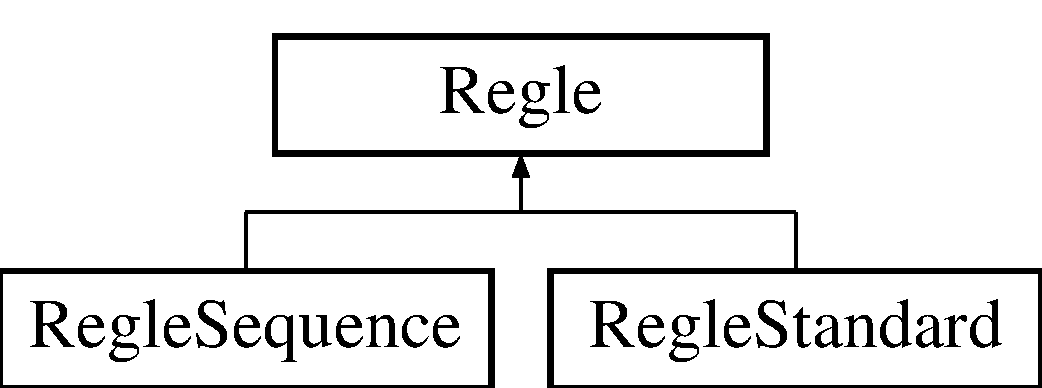
\includegraphics[height=2.000000cm]{class_regle}
\end{center}
\end{figure}
\subsection*{Fonctions membres publiques}
\begin{DoxyCompactItemize}
\item 
\hypertarget{class_regle_a1c56ca5ad1d119d177239c35b0e4410b}{virtual vector$<$ \hyperlink{class_noeud}{Noeud} $\ast$ $>$ {\bfseries appliquer} (\hyperlink{class_parser}{Parser} $\ast$p)=0}\label{class_regle_a1c56ca5ad1d119d177239c35b0e4410b}

\end{DoxyCompactItemize}


La documentation de cette classe a été générée à partir du fichier suivant \-:\begin{DoxyCompactItemize}
\item 
grammaire/regles/Regle.\-h\end{DoxyCompactItemize}

\hypertarget{class_regle_sequence}{\section{Référence de la classe Regle\-Sequence}
\label{class_regle_sequence}\index{Regle\-Sequence@{Regle\-Sequence}}
}
Graphe d'héritage de Regle\-Sequence\-:\begin{figure}[H]
\begin{center}
\leavevmode
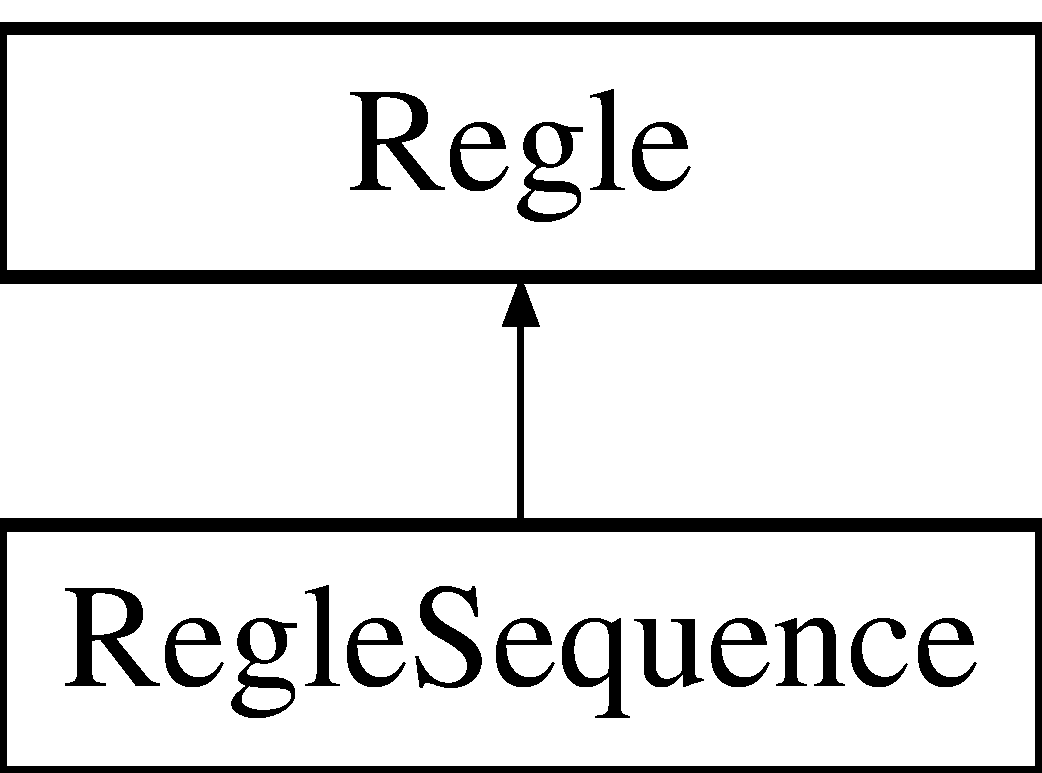
\includegraphics[height=2.000000cm]{class_regle_sequence}
\end{center}
\end{figure}
\subsection*{Fonctions membres publiques}
\begin{DoxyCompactItemize}
\item 
\hyperlink{class_regle_sequence_a7cba8d2491d2f5c1854f6d9e40db018d}{Regle\-Sequence} (string nom, string type)
\begin{DoxyCompactList}\small\item\em Crée une règle de type séquence. \end{DoxyCompactList}\item 
vector$<$ \hyperlink{class_noeud}{Noeud} $\ast$ $>$ \hyperlink{class_regle_sequence_a523224e9cbace57e6a96a957b8fb04c4}{appliquer} (\hyperlink{class_parser}{Parser} $\ast$p)
\begin{DoxyCompactList}\small\item\em Renvoie les noeuds résultants de l'application de la règle à l'état courant du parser. \end{DoxyCompactList}\item 
void \hyperlink{class_regle_sequence_af30c68a9b9a2358e248d5f4edc4a4074}{init} ()
\begin{DoxyCompactList}\small\item\em Initialise la règle pour le parsing (doit être appelé avant chaque nouveau parsing). \end{DoxyCompactList}\end{DoxyCompactItemize}
\subsection*{Attributs publics}
\begin{DoxyCompactItemize}
\item 
vector$<$ \hyperlink{class_condition_unique}{Condition\-Unique} $\ast$ $>$ \hyperlink{class_regle_sequence_a7e254237c15832f3b5e79fef57fdac54}{conditions}
\begin{DoxyCompactList}\small\item\em Les conditions portant sur le membre droit (par exemple, chaque marche doit mesurer plus de 30 cm). \end{DoxyCompactList}\item 
vector$<$ \hyperlink{class_condition_adj}{Condition\-Adj} $\ast$ $>$ \hyperlink{class_regle_sequence_a0b99e9875a308dac54e99358d5d2a712}{cond\-Succ\-Adj}
\begin{DoxyCompactList}\small\item\em Les conditions d'adjacence entre attributs de deux éléments consécutifs. \end{DoxyCompactList}\item 
vector$<$ \hyperlink{class_condition_egal}{Condition\-Egal} $\ast$ $>$ \hyperlink{class_regle_sequence_aeb7ff397207904508a29b2f15c6841f1}{cond\-Succ\-Egal}
\begin{DoxyCompactList}\small\item\em Les conditions d'égalité entre attributs de deux éléments consécutifs. \end{DoxyCompactList}\end{DoxyCompactItemize}
\subsection*{Attributs privés}
\begin{DoxyCompactItemize}
\item 
\hypertarget{class_regle_sequence_aefc0acf54c76f95a15080df4996ce296}{string {\bfseries type}}\label{class_regle_sequence_aefc0acf54c76f95a15080df4996ce296}

\item 
\hypertarget{class_regle_sequence_ab57ac6215025b673691010b0a2a57b87}{string {\bfseries nom}}\label{class_regle_sequence_ab57ac6215025b673691010b0a2a57b87}

\item 
\hypertarget{class_regle_sequence_af43a1ef4bd41eba1ad989831df6831cf}{set$<$ \hyperlink{class_element}{Element} $\ast$ $>$ {\bfseries elements}}\label{class_regle_sequence_af43a1ef4bd41eba1ad989831df6831cf}

\item 
\hypertarget{class_regle_sequence_aa3dbd3a9d1d025918a4cd38e4ae2505c}{set$<$ \hyperlink{class_noeud}{Noeud} $\ast$ $>$ {\bfseries deja\-Traites}}\label{class_regle_sequence_aa3dbd3a9d1d025918a4cd38e4ae2505c}

\item 
\hypertarget{class_regle_sequence_ac76b51a73c43c3122b43f0782e3d3355}{map$<$ \hyperlink{class_condition_adj}{Condition\-Adj} $\ast$, map\\*
$<$ \hyperlink{class_polygone}{Polygone} $\ast$, set$<$ \hyperlink{class_element}{Element} $\ast$ $>$ $>$ $>$ {\bfseries table\-\_\-debuts}}\label{class_regle_sequence_ac76b51a73c43c3122b43f0782e3d3355}

\item 
\hypertarget{class_regle_sequence_a57b2f9884234276fa004d006a60b7653}{map$<$ \hyperlink{class_condition_adj}{Condition\-Adj} $\ast$, map\\*
$<$ \hyperlink{class_polygone}{Polygone} $\ast$, set$<$ \hyperlink{class_element}{Element} $\ast$ $>$ $>$ $>$ {\bfseries table\-\_\-fins}}\label{class_regle_sequence_a57b2f9884234276fa004d006a60b7653}

\item 
\hypertarget{class_regle_sequence_a6fc2e70a5a7715ebd8058f77f9f52eb8}{map$<$ \hyperlink{class_condition_egal}{Condition\-Egal} $\ast$, map\\*
$<$ void $\ast$, set$<$ \hyperlink{class_element}{Element} $\ast$ $>$ $>$ $>$ {\bfseries table\-\_\-eg\-\_\-debuts}}\label{class_regle_sequence_a6fc2e70a5a7715ebd8058f77f9f52eb8}

\item 
\hypertarget{class_regle_sequence_ae4af3c30ff37df35b459ce338c7293c9}{map$<$ \hyperlink{class_condition_egal}{Condition\-Egal} $\ast$, map\\*
$<$ void $\ast$, set$<$ \hyperlink{class_element}{Element} $\ast$ $>$ $>$ $>$ {\bfseries table\-\_\-eg\-\_\-fins}}\label{class_regle_sequence_ae4af3c30ff37df35b459ce338c7293c9}

\end{DoxyCompactItemize}


\subsection{Documentation des constructeurs et destructeur}
\hypertarget{class_regle_sequence_a7cba8d2491d2f5c1854f6d9e40db018d}{\index{Regle\-Sequence@{Regle\-Sequence}!Regle\-Sequence@{Regle\-Sequence}}
\index{Regle\-Sequence@{Regle\-Sequence}!RegleSequence@{Regle\-Sequence}}
\subsubsection[{Regle\-Sequence}]{\setlength{\rightskip}{0pt plus 5cm}{\bf Regle\-Sequence\-::\-Regle\-Sequence} (
\begin{DoxyParamCaption}
\item[{string}]{nom, }
\item[{string}]{type}
\end{DoxyParamCaption}
)}}\label{class_regle_sequence_a7cba8d2491d2f5c1854f6d9e40db018d}


Crée une règle de type séquence. 


\begin{DoxyParams}{Paramètres}
{\em nom} & Le nom du non-\/terminal. \\
\hline
{\em type} & Le type répété (i.\-e. apparaissant en partie droite de la règle). \\
\hline
\end{DoxyParams}


\subsection{Documentation des fonctions membres}
\hypertarget{class_regle_sequence_a523224e9cbace57e6a96a957b8fb04c4}{\index{Regle\-Sequence@{Regle\-Sequence}!appliquer@{appliquer}}
\index{appliquer@{appliquer}!RegleSequence@{Regle\-Sequence}}
\subsubsection[{appliquer}]{\setlength{\rightskip}{0pt plus 5cm}vector$<$ {\bf Noeud} $\ast$ $>$ {\bf Regle\-Sequence\-::appliquer} (
\begin{DoxyParamCaption}
\item[{{\bf Parser} $\ast$}]{p}
\end{DoxyParamCaption}
)\hspace{0.3cm}{\ttfamily  \mbox{[}virtual\mbox{]}}}}\label{class_regle_sequence_a523224e9cbace57e6a96a957b8fb04c4}


Renvoie les noeuds résultants de l'application de la règle à l'état courant du parser. 


\begin{DoxyParams}{Paramètres}
{\em parser} & Le parser de la grammaire en cours d'exécutino \\
\hline
\end{DoxyParams}
\begin{DoxyReturn}{Renvoie}
Les noeuds créés. 
\end{DoxyReturn}


Implémente \hyperlink{class_regle}{Regle}.

\hypertarget{class_regle_sequence_af30c68a9b9a2358e248d5f4edc4a4074}{\index{Regle\-Sequence@{Regle\-Sequence}!init@{init}}
\index{init@{init}!RegleSequence@{Regle\-Sequence}}
\subsubsection[{init}]{\setlength{\rightskip}{0pt plus 5cm}void {\bf Regle\-Sequence\-::init} (
\begin{DoxyParamCaption}
{}
\end{DoxyParamCaption}
)}}\label{class_regle_sequence_af30c68a9b9a2358e248d5f4edc4a4074}


Initialise la règle pour le parsing (doit être appelé avant chaque nouveau parsing). 

Réinitialise les structures utilisées lors du parsing. 

\subsection{Documentation des données membres}
\hypertarget{class_regle_sequence_a7e254237c15832f3b5e79fef57fdac54}{\index{Regle\-Sequence@{Regle\-Sequence}!conditions@{conditions}}
\index{conditions@{conditions}!RegleSequence@{Regle\-Sequence}}
\subsubsection[{conditions}]{\setlength{\rightskip}{0pt plus 5cm}vector$<${\bf Condition\-Unique}$\ast$$>$ {\bf Regle\-Sequence\-::conditions}}}\label{class_regle_sequence_a7e254237c15832f3b5e79fef57fdac54}


Les conditions portant sur le membre droit (par exemple, chaque marche doit mesurer plus de 30 cm). 

\hypertarget{class_regle_sequence_a0b99e9875a308dac54e99358d5d2a712}{\index{Regle\-Sequence@{Regle\-Sequence}!cond\-Succ\-Adj@{cond\-Succ\-Adj}}
\index{cond\-Succ\-Adj@{cond\-Succ\-Adj}!RegleSequence@{Regle\-Sequence}}
\subsubsection[{cond\-Succ\-Adj}]{\setlength{\rightskip}{0pt plus 5cm}vector$<${\bf Condition\-Adj}$\ast$$>$ {\bf Regle\-Sequence\-::cond\-Succ\-Adj}}}\label{class_regle_sequence_a0b99e9875a308dac54e99358d5d2a712}


Les conditions d'adjacence entre attributs de deux éléments consécutifs. 

\hypertarget{class_regle_sequence_aeb7ff397207904508a29b2f15c6841f1}{\index{Regle\-Sequence@{Regle\-Sequence}!cond\-Succ\-Egal@{cond\-Succ\-Egal}}
\index{cond\-Succ\-Egal@{cond\-Succ\-Egal}!RegleSequence@{Regle\-Sequence}}
\subsubsection[{cond\-Succ\-Egal}]{\setlength{\rightskip}{0pt plus 5cm}vector$<${\bf Condition\-Egal}$\ast$$>$ {\bf Regle\-Sequence\-::cond\-Succ\-Egal}}}\label{class_regle_sequence_aeb7ff397207904508a29b2f15c6841f1}


Les conditions d'égalité entre attributs de deux éléments consécutifs. 



La documentation de cette classe a été générée à partir des fichiers suivants \-:\begin{DoxyCompactItemize}
\item 
grammaire/regles/Regle\-Sequence.\-h\item 
grammaire/regles/Regle\-Sequence.\-cpp\end{DoxyCompactItemize}

\hypertarget{class_regle_standard}{\section{Référence de la classe Regle\-Standard}
\label{class_regle_standard}\index{Regle\-Standard@{Regle\-Standard}}
}
Graphe d'héritage de Regle\-Standard\-:\begin{figure}[H]
\begin{center}
\leavevmode
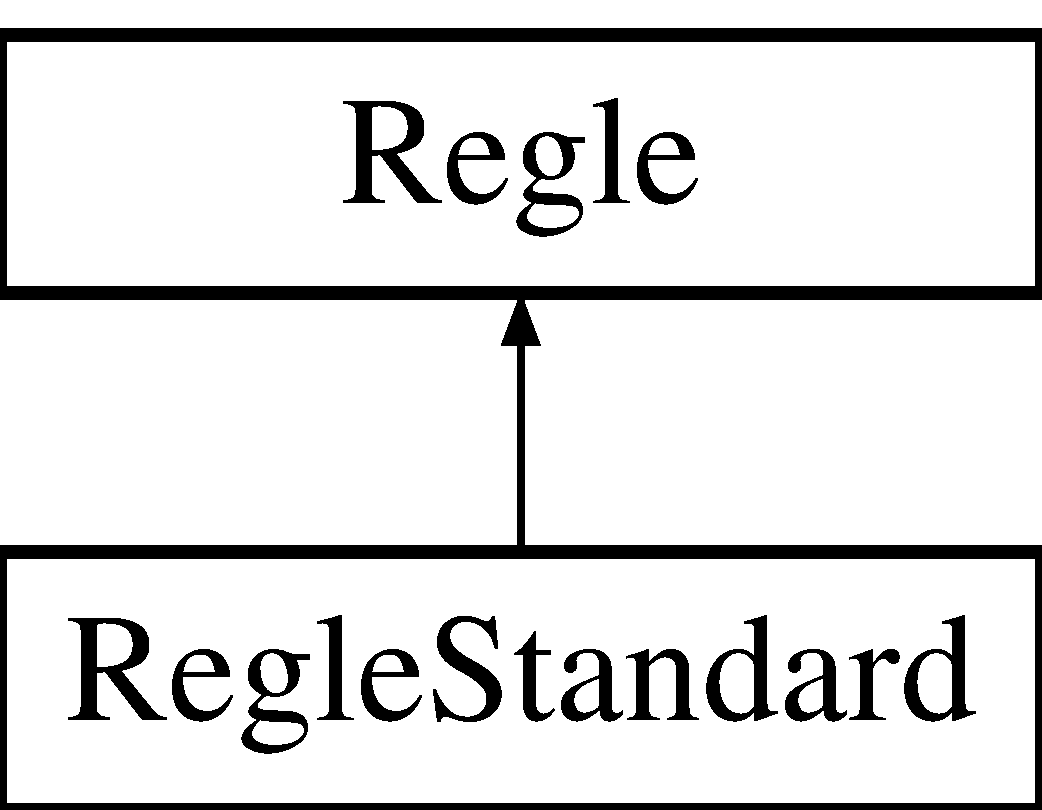
\includegraphics[height=2.000000cm]{class_regle_standard}
\end{center}
\end{figure}
\subsection*{Fonctions membres publiques}
\begin{DoxyCompactItemize}
\item 
\hypertarget{class_regle_standard_a31ce3a86daa4053c28d0ce01a5e7987b}{{\bfseries Regle\-Standard} (string nom, vector$<$ string $>$ membres\-Droits, vector$<$ \hyperlink{class_condition}{Condition} $\ast$ $>$ conditions)}\label{class_regle_standard_a31ce3a86daa4053c28d0ce01a5e7987b}

\item 
\hypertarget{class_regle_standard_a1f7a35bb71c7ca8bcef317c5bb05bf05}{vector$<$ \hyperlink{class_noeud}{Noeud} $\ast$ $>$ {\bfseries appliquer} (\hyperlink{class_parser}{Parser} $\ast$p)}\label{class_regle_standard_a1f7a35bb71c7ca8bcef317c5bb05bf05}

\end{DoxyCompactItemize}
\subsection*{Attributs privés}
\begin{DoxyCompactItemize}
\item 
\hypertarget{class_regle_standard_a41918ffb7f2a22a292159d4ce93958e1}{string {\bfseries nom}}\label{class_regle_standard_a41918ffb7f2a22a292159d4ce93958e1}

\item 
\hypertarget{class_regle_standard_aaf9eca4d8e384a527cc164d0fea9be8a}{vector$<$ string $>$ {\bfseries membres\-Droits}}\label{class_regle_standard_aaf9eca4d8e384a527cc164d0fea9be8a}

\item 
\hypertarget{class_regle_standard_a9cdaa6a3143dfdfad1cfb3dc7363ce44}{vector$<$ \hyperlink{class_condition}{Condition} $\ast$ $>$ {\bfseries conditions}}\label{class_regle_standard_a9cdaa6a3143dfdfad1cfb3dc7363ce44}

\end{DoxyCompactItemize}


La documentation de cette classe a été générée à partir des fichiers suivants \-:\begin{DoxyCompactItemize}
\item 
grammaire/regles/Regle\-Standard.\-h\item 
grammaire/regles/Regle\-Standard.\-cpp\end{DoxyCompactItemize}

\hypertarget{class_terminal}{\section{Référence de la classe Terminal}
\label{class_terminal}\index{Terminal@{Terminal}}
}
Graphe d'héritage de Terminal\-:\begin{figure}[H]
\begin{center}
\leavevmode
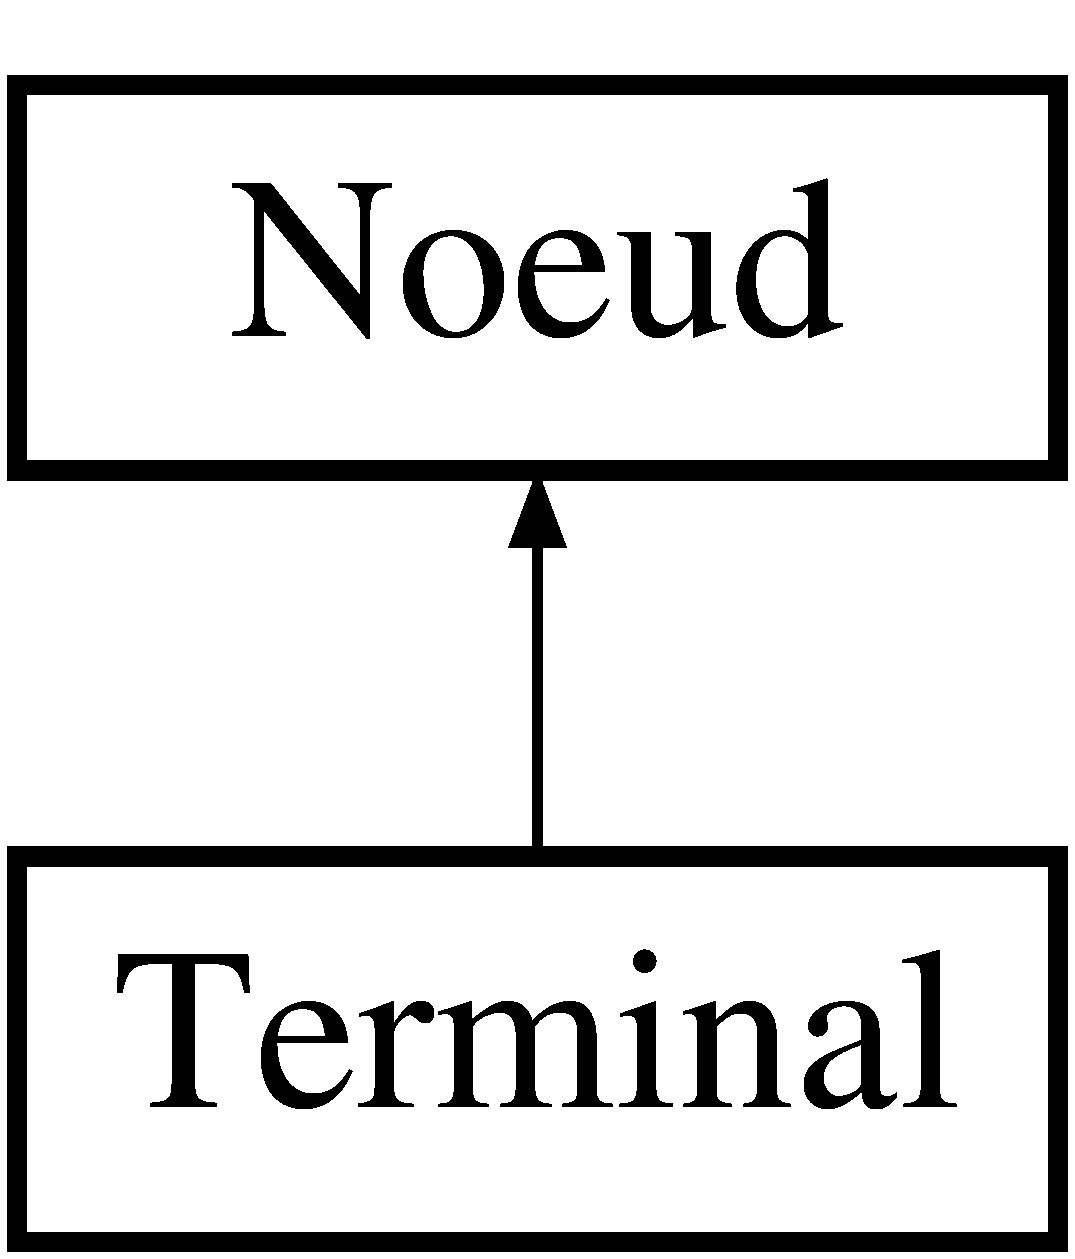
\includegraphics[height=2.000000cm]{class_terminal}
\end{center}
\end{figure}
\subsection*{Fonctions membres publiques}
\begin{DoxyCompactItemize}
\item 
\hypertarget{class_terminal_a221ebc6bdede0a9a032a0f0a98fb6e52}{{\bfseries Terminal} (\hyperlink{class_polygone}{Polygone} $\ast$polygone, int number)}\label{class_terminal_a221ebc6bdede0a9a032a0f0a98fb6e52}

\item 
\hypertarget{class_terminal_a3a91bb783ae607efd0a42b2707ca6493}{vector$<$ \hyperlink{class_noeud}{Noeud} $\ast$ $>$ {\bfseries get\-Enfants} ()}\label{class_terminal_a3a91bb783ae607efd0a42b2707ca6493}

\item 
\hypertarget{class_terminal_a07e1cf40f0889f07b3b9ec78e29b480b}{string {\bfseries get\-Type} ()}\label{class_terminal_a07e1cf40f0889f07b3b9ec78e29b480b}

\item 
\hypertarget{class_terminal_a522310dd9ed87cb320c45c109610ac12}{bool {\bfseries equals} (\hyperlink{class_noeud}{Noeud} $\ast$n)}\label{class_terminal_a522310dd9ed87cb320c45c109610ac12}

\end{DoxyCompactItemize}
\subsection*{Attributs privés}
\begin{DoxyCompactItemize}
\item 
\hypertarget{class_terminal_a4cdd1bfc11e15f5b287ff3e4de29bc9e}{string {\bfseries type}}\label{class_terminal_a4cdd1bfc11e15f5b287ff3e4de29bc9e}

\end{DoxyCompactItemize}


La documentation de cette classe a été générée à partir des fichiers suivants \-:\begin{DoxyCompactItemize}
\item 
grammaire/parsing/Terminal.\-h\item 
grammaire/parsing/Terminal.\-cpp\end{DoxyCompactItemize}

\hypertarget{class_vec3}{\section{Référence de la classe Vec3}
\label{class_vec3}\index{Vec3@{Vec3}}
}
\subsection*{Fonctions membres publiques}
\begin{DoxyCompactItemize}
\item 
\hypertarget{class_vec3_a842ccdcdb2b4c7ca7cef20e6e786a231}{{\bfseries Vec3} (float x, float y, float z)}\label{class_vec3_a842ccdcdb2b4c7ca7cef20e6e786a231}

\item 
\hypertarget{class_vec3_ab0166900ca119ef6e3b7d928cc40fe4a}{{\bfseries Vec3} (\hyperlink{structobj__vector}{obj\-\_\-vector} $\ast$v)}\label{class_vec3_ab0166900ca119ef6e3b7d928cc40fe4a}

\item 
\hypertarget{class_vec3_a428e2ccce86f110a37f3291825f05e8d}{{\bfseries Vec3} (\hyperlink{structobj__vector}{obj\-\_\-vector} $\ast$p1, \hyperlink{structobj__vector}{obj\-\_\-vector} $\ast$p2)}\label{class_vec3_a428e2ccce86f110a37f3291825f05e8d}

\item 
\hypertarget{class_vec3_a4931806f11adc8e9b5a9b6f011b0ea4f}{const \hyperlink{class_vec3}{Vec3} {\bfseries operator$^\wedge$} (const \hyperlink{class_vec3}{Vec3} \&other) const }\label{class_vec3_a4931806f11adc8e9b5a9b6f011b0ea4f}

\item 
\hypertarget{class_vec3_ac036ec1f148a700490aae0b8958809fa}{const \hyperlink{class_vec3}{Vec3} {\bfseries operator-\/} (const \hyperlink{class_vec3}{Vec3} \&other) const }\label{class_vec3_ac036ec1f148a700490aae0b8958809fa}

\item 
\hypertarget{class_vec3_a21d1b56373372cdbe01345af63b8e274}{float {\bfseries operator$\ast$} (const \hyperlink{class_vec3}{Vec3} \&other) const }\label{class_vec3_a21d1b56373372cdbe01345af63b8e274}

\item 
\hypertarget{class_vec3_a4081cea9cbb7668d9ac5666072cacda1}{bool {\bfseries operator==} (const \hyperlink{class_vec3}{Vec3} \&other) const }\label{class_vec3_a4081cea9cbb7668d9ac5666072cacda1}

\item 
\hypertarget{class_vec3_a3a6631559d1d36eaf34ca586ce86ede1}{void {\bfseries normalize} ()}\label{class_vec3_a3a6631559d1d36eaf34ca586ce86ede1}

\item 
\hypertarget{class_vec3_a85037fb497ccaf866867da14f43b63c5}{float {\bfseries norm} () const }\label{class_vec3_a85037fb497ccaf866867da14f43b63c5}

\end{DoxyCompactItemize}
\subsection*{Attributs publics}
\begin{DoxyCompactItemize}
\item 
\hypertarget{class_vec3_a2814580e9b9372738c0a61197ea46b51}{float {\bfseries x}}\label{class_vec3_a2814580e9b9372738c0a61197ea46b51}

\item 
\hypertarget{class_vec3_abc1d241232cb04aa98217a942402ae68}{float {\bfseries y}}\label{class_vec3_abc1d241232cb04aa98217a942402ae68}

\item 
\hypertarget{class_vec3_a64f3f00cd2dd9076999eeb2f05210388}{float {\bfseries z}}\label{class_vec3_a64f3f00cd2dd9076999eeb2f05210388}

\end{DoxyCompactItemize}


La documentation de cette classe a été générée à partir du fichier suivant \-:\begin{DoxyCompactItemize}
\item 
geometrie/Vec3.\-h\end{DoxyCompactItemize}

\printindex
\end{document}
